\section*{What Language for Our Language?}

Programming can be seen as an art, where programming languages serve as a kind of paintbrush. There are several languages, or paintbrushes, we could use, e.g., Python, Java, C++, Rust, and others, but we will use the C programming language. C is what many consider a ``medium-level''\index{medium-level} language: one that is higher-level\index{high-level} than mnemonic-driven instructions and binary encoding\index{binary}, but lower-level\index{low-level} insofar as its close interaction with the computer hardware. Experienced computer scientists and programmers may view our decision to use C as rather odd, since it allows beginners to fall into bad programming practice traps and is significantly more ``dangerous'' than many others of its kind.\footnote{By ``dangerous'', we mean its security vulnerabilities.} We argue, however, that C is a simple and small programming language, containing few keywords and programming abstractions\index{programming abstraction}. Furthermore, C is a \textit{procedural}\index{procedural} programming language, which means that it follows a step-by-step execution model. This aligns well with how beginners generally think and approach problem solving. Procedural programming allows beginners to grasp the concept of sequential execution, making it easier to understand the logic behind their programs. Finally, C serves as a solid foundation for learning other programming languages, as many modern languages, such as those we listed above, have C as their underlying influence.

In this section, we finally start writing code! In addition, we will reintroduce some concepts that we discussed from Chapters~\ref{chapter-maths}, \ref{chapter-datastructures}, and ~\ref{chapter-languages}. This time, however, we emphasize their relationships to programming as opposed to focusing solely on their theoretical potential.

\subsubsection*{Hello World!}

Every programming introduction uses the famous, ``Hello World!''\index{hello world} program of some variety, and our textbook is no exception. Refer to Appendix~\ref{appendix-project-setup} to set up your programming environment.

\begin{cloast}[main.c]{Hello World Program}
\begin{lstlisting}[language=MyC]
#include <stdio.h>

int main(void) {
 printf("Hello, world!");
 return 0;
}
\end{lstlisting}
\tcblower
\begin{lstlisting}[language=MyOutput]
Hello, world!
\end{lstlisting}
\end{cloast}

What does this program do? We will go line-by-line in our analysis.

Line 1 includes functions from the standard input and output\index{standard input}\index{standard output} library in C. This contains several functions that allow programmers to output information to the console, files, as well as read information from the user.

Line 3 declares a function called \texttt{main} that has no arguments which returns a value of type \texttt{int}. A function, as we can recall from Chapter~\ref{chapter-maths}, is a series of computations to perform a task. In C, every program needs a \texttt{main} function. There are some slight variations that \texttt{main} may take the form, but for now, we consider those irrelevant. There is also an opening curly brace \texttt{\{}. All functions in C require a pair of opening and closing braces \texttt{\{}, \texttt{\}} to designate the \textit{body} of a function, i.e., where the steps to perform a task resides. 

Line 4 calls the \texttt{printf} function with the string argument ``\texttt{Hello, world!}''. The \texttt{printf} function formats output information to the console, and can be a bit complex for people to wrap their heads around initially. We will explore this function a bit more later in our C primer, but for now, we can just make note of the fact that it outputs a string to the console.

Line 5 says that the \ttt{main} function returns a value of \texttt{0}. For all intents and purposes of our adventure in this textbook, the fact that \texttt{main} returns a value at all is somewhat superfluous. For completeness, however, we will say that \texttt{main} returns an integer value based on the ``state'' of the program. In other words, returning a value of \texttt{0} from \texttt{main} indicates that the program, or \texttt{main} function for that matter, terminated successfully. If by chance there was an error that occurred somewhere, we could return a nonzero integer such as \texttt{1} or \texttt{-1}.

Finally, line 6 has the closing brace for the \texttt{main} function.

\subsubsection*{Natural Recursion}
In Chapter~\ref{chapter-maths}, we introduced the notion of \textit{recursive functions}\index{recursive function}, i.e., functions that call themselves. To gently introduce the notion of recursive functions in the C programming language, we will write some primitive operations via \textit{natural recursion}\index{natural recursion}. Natural recursion is a type of recursion that operates over the natural numbers, i.e., $\mathbb{N}$, or numbers from $\{0,\;1,\;2,\;3,\;\ldots\}$. Since such a concept is rather abstract at first glance, let us illustrate this with what appears to be a simple example: $\textsf{Add}(x,\;y)$.

\subsubsection*{Addition with Natural Recursion}
How do we add two natural numbers $x$ and $y$? If we actually sit down and think about how addition works, there are almost certainly some shortcuts people take. For instance, if $x=19$ and $y=43$, we can say that $x$ is very close to $20$, so we can simply add $20$ to $y$ and subtract one. Though, we are still missing this notion of addition. If we wish to think about this problem recursively, it would be wise to introduce a base case.

What happens if we add zero to any natural number? We simply get back the natural number. So, this can be treated as our base case\index{base case}. What about the recursive step\index{recursive step}? Let us assume, for the sake of constructing the solution to a larger problem, that we understand the idea behind adding exactly one to a value and subtracting exactly one to a value. If we have two natural numbers $x$ and $y$, we can recursively compute the sum of $x$ and $y$ by taking the successor\index{successor} of $x$ and subtracting one from $y$. The successor of some natural number $n$ is equal to $n\;+\;1$, using the function $\textsf{Succ}$. E.g., $\textsf{Succ}(5)=6$. So, our definition of addition, $\textsf{Add}(x,\;y) = \textsf{Succ}(\textsf{Add}(x,\;y\;-\;1))$. 
\begin{align*}
    &\text{Base case: If }y\text{ is }0\text{, return } x.\\
    &\text{Recursive step: Return }1 + \textsf{Add}(x,\;y\;-\;1)
\end{align*}
Like always, a good motivation for understanding comes through an example. Using the preceding base case and recursive step, let us add $x = 9$, and $y = 3$.
\begin{enumerate}[label=(\roman*)]
    \item First, we call $\textsf{Add}(9,\;3)$. Is 3 equal to 0? Clearly not, so we do not return 9. We return $1 + \textsf{Add}(9,\;2)$.
    \item Is 2 equal to 0? Clearly not, so we do not return 9. We return $1 + \textsf{Add}(9,\;1)$.
    \item Is 1 equal to 0? Clearly not, so we do not return 9. We return $1 + \textsf{Add}(9,\;0)$.
    \item Is 0 equal to 0? Clearly, so we return $9$. We now begin the process of reversing through the recursive calls since we reached our base case.
    \item Previously, we had $1 + \textsf{Add}(9,\;0)$. We now know that $\textsf{Add}(9,\;0) = 9$, so we return $1 + 9 = 10$.
    \item Previously, we had $1 + \textsf{Add}(9,\;1)$. We now know that $\textsf{Add}(9,\;1) = 10$, so we return $1 + 10 = 11$.
    \item Previously, we had $1 + \textsf{Add}(9,\;2)$. We now know that $\textsf{Add}(9,\;2) = 11$, so we return $1 + 11 = 12$.
    \item We are out of recursive calls, so our final result is $12$.
\end{enumerate}
As shown above, the function returns $12$ for $x=9$ and $y=3$, which is correct, as $9 + 3 = 12$. Let us now write some C code to replicate this algorithm. Note that we will only list the function and not the \texttt{main} function or headers.

\begin{cl}[main.c]{Naturally-Recursive Addition}
\begin{lstlisting}[language=MyC]
int add(int x, int y) {
 if (0 == y) { return x; }
 else { return 1 + add(x, y - 1); }
}
\end{lstlisting}
\end{cl}

An important note about computing $\textsf{Add}(x,\;y)$ via natural recursion is that this algorithm does not work if $y$ is any negative integer. Our base case checks to see if $y$ is equal to zero. The current approach subtracts one from $y$ every time we recursively call \textsf{Add}. This means that $y$ will never be zero, and is therefore stuck in infinite recursion.

\subsubsection*{Multiplication with Natural Recursion}

Now that we understand the notion of natural recursion with addition, we should write a program to multiply two natural numbers. When we multiply two natural numbers $x$ and $y$ using natural recursion, we define multiplication in terms of addition. Namely, we add $x$ to itself $y$ times. Our base case is trivial: any number multiplied by zero results in zero. Then, we add recursively add $n$ to the result of invoking \textsf{Mult}.
\begin{align*}
    &\text{Base case: If }y\text{ is }0\text{, return }0\text{.}\\
    &\text{Recursive step: Return $\textsf{Add}(x,\;\textsf{Mult}(x,\;y\;-\;1)))$}
\end{align*}
Again, let us use a simple example. Suppose we wish to multiply $x=8$ and $y=4$.
\begin{enumerate}[label=(\roman*)]
    \item First, we call $\textsf{Mult}(8,\;4)$. Is $4$ equal to $0$? Clearly not, so we do not return $0$. We return $\textsf{Add}(8,\;\textsf{Mult}(8,\;3))$.
    \item Is $3$ equal to $0$? Clearly not, so we do not return $0$. We return $\textsf{Add}(8,\;\textsf{Mult}(8,\;2))$.
    \item Is $2$ equal to $0$? Clearly not, so we do not return $0$. We return $\textsf{Add}(8,\;\textsf{Mult}(8,\;1))$.
    \item Is $1$ equal to $0$? Clearly not, so we do not return $0$. We return $\textsf{Add}(8,\;\textsf{Mult}(8,\;0))$.
    \item Is $0$ equal to $0$? Clearly, so we return $0$. We now begin the process of reversing through the recursive calls since we reached our base case.
    \item Previously, we had $\textsf{Add}(8,\;\textsf{Mult}(8,\;0))$. We now know that $\textsf{Mult}(8,\;0)=0$, so we return $8+0=8$.
    \item Previously, we had $\textsf{Add}(8,\;\textsf{Mult}(8,\;1))$. We now know that $\textsf{Mult}(8,\;1)=8$, so we return $8+8=16$.
    \item Previously, we had $\textsf{Add}(8,\;\textsf{Mult}(8,\;2))$. We now know that $\textsf{Mult}(8,\;2)=16$, so we return $8+16=24$.
    \item Previously, we had $\textsf{Add}(8,\;\textsf{Mult}(8,\;3))$. We now know that $\textsf{Mult}(8,\;3)=24$, so we return $8+24=32$.
    \item We are out of recursive calls, so our final result is $32$.
\end{enumerate}

\begin{cl}[main.c]{Naturally-Recursive Multiplication}
\begin{lstlisting}[language=MyC]
int mult(int x, int y) { 
 if (0 == y) { return 0; }
 else { return add(x, mult(x, y\;-\;1)); }
}
\end{lstlisting}
\end{cl}

\subsubsection*{Exponentials\index{exponential} with Natural Recursion}

We will derive another naturally-recursive function: $\textsf{Pow}(x,\;y)$, which is equivalent to $x^y$, or $x$ multiplied by itself $y$ times. As before, we need a base case and a recursive step. Assuming $x$ and $y$ are natural numbers, then $x^0=1$ should certainly be our base case. The recursive step is fortunately only slightly harder: $x^y = x \cdot x^{(y\;-\;1)}$. Written out formally, we can, and should, express exponentiation in terms of \textsf{Mult}:
\begin{align*}
    &\text{Base case: If }y\text{ is }0\text{, return 1.}\\
    &\text{Recursive step: Return }\textsf{Mult}(x,\;\textsf{Pow}(x,\;y\;-\;1)).
\end{align*}

\noindent And the code is just a retailing of the formal definition:

\begin{cl}[main.c]{Naturally-Recursive Exponentiation}
\begin{lstlisting}[language=MyC]
int pow(int x, int y) {
 if (0 == y) { return 1; }
 else { return mult(x, pow(x, y - 1)); }
}
\end{lstlisting}
\end{cl}

\subsubsection*{Factorial\index{factorial} with Natural Recursion}

Let us ramp things up a bit more and write a slightly harder function, which \texttt{main} will invoke, i.e., call. We saw \textsf{fact($n$)}, a function that computes the factorial of a positive integer $n$, in Chapter~\ref{chapter-maths}. We noted the base case and the recursive step of \textsf{fact}.

\begin{align*}
    &\text{Base case: If }n\leq{1}\text{, return }1.\\
    &\text{Recursive step: Return }n \cdot \textsf{fact}(n-1)
\end{align*}

In C, it is quite trivial to replicate this behavior! We can use the conditional \texttt{if} to mimic the base case. Unlike the section on natural recursion, we will first write the code to compute $\textsf{fact}(n)$, then walk through a computation example.

\begin{clo}[main.c]{Naturally-Recursive Factorial}
\begin{lstlisting}[language=MyC]
#include <stdio.h>

int fact(int n) {
 if (n <= 1) { return 1; }
 else { return n * fact(n - 1); }
}

int main() {
 int x = 6;
 printf("The factorial of %d is %d\n", x, fact(x));
 return 0;
}
\end{lstlisting}
\tcblower
\begin{lstlisting}[language=MyOutput]
The factorial of 
6 is 720
\end{lstlisting}
\end{clo}

Inside the \texttt{main} function, we declare an integer $x$ with the value of $6$. Variables serve as placeholders for a value. This means that wherever we refer to $x$, the program will interpret this as the integer $6$.

Our \texttt{printf}\index{\ttt{printf}} statement looks a bit complex now, so what did we do? Fear not, however, as even though it appears difficult to understand, its behavior is entirely predictable. The first argument to \texttt{printf} is what we call a format string. A format string is a string that has placeholders for data. These placeholders can represent anything: integers, floating-point values, characters, strings, memory addresses, or whatever we desire! In this case, we are printing out the characters ``\texttt{The factorial of }'', then we encounter a \texttt{\%d}. This is a placeholder for a value. Since it is the first placeholder in this string, it is going to search through the rest of the arguments to \texttt{printf}, i.e., \texttt{x} and \texttt{fact(x)}, and display the value of the first argument, being the value of \texttt{x}. It then prints the characters ``\texttt{ is }'', followed by another placeholder \texttt{\%d}.\footnote{Note that there is another special character `\texttt{\textbackslash{n}}' This causes the program to return to the next line. It is akin to pressing ``Enter''.} Since this is the second placeholder, it will extract the value of \textsf{fact}$(x)$ This, however, is a function, so it will need to compute the value of \textsf{fact}$(x)$before printing it out.

Let us trace through a computation of \textsf{fact}$(3)$ to clarify some certainly-present confusion about recursion.\footnote{We use $3$ instead of $6$ to shorten the redundancy of the explanation.}

\begin{enumerate}[label=(\roman*)]
    \item First, we call $\textsf{fact}(3)$ from \texttt{main}. We ask, ``Is $3$ less than or equal to 1?'' Clearly not, so we do not execute the code inside the \texttt{if} body. We compute $3 \cdot\textsf{fact}(2)$.
    \item $\textsf{fact}(2)$ is called. We ask, ``Is $2$ less than or equal to $1$?'' Clearly not, so we do not execute the code inside the \texttt{if} body. We then compute $2 \cdot \textsf{fact}(1)$.
    \item $\textsf{fact}(1)$ is called. We ask, ``Is $1$ less than or equal to $1$?'' Clearly this is true, so we execute the code inside the \texttt{if} body. We return 1. We now begin the process of reversing through the recursive calls since we reached our base case.
    \item Previously, we had $2 \cdot \textsf{fact}(1)$. We now know $\textsf{fact}(1)=1$, so we return $2\cdot{1}=2$.
    \item Previously, we had $3 \cdot \textsf{fact}(2)$. We now know $\textsf{fact}(2)=2$, so we return $3\cdot{2}=6$.
    \item We are out of recursive calls, so our final result is $6$.
\end{enumerate}

As shown above, the function returns $6$ for $n=3$, which is correct, as $3!=3\cdot{2}\cdot{1}=6$.

\subsubsection*{Computing Catalan Numbers with Natural Recursion}

The \textit{catalan numbers}\index{catalan numbers} are a sequence of natural numbers that fall ``nicely'' into a recursive formula. This formula may look a little scary, but it is nothing more than another form of natural recursion.\footnote{While their uses are not important for us, we note that they aid in combinatorics, i.e., permutations.}
\begin{align*}
    C_0 &= 1\\
    C_n &= \dfrac{2(2n-1)}{n\;+\;1}\cdot{C_{n-1}}
\end{align*}
\begin{cl}[main.c]{Naturally-Recursive Catalan Numbers}
\begin{lstlisting}[language=MyC]
int catalan(int n) {
 if (n == 0) { return 1; }
 else { return (int) ((2.0 * (2 * n - 1)) / (n + 1)) * catalan(n - 1); }
}
\end{lstlisting}
\end{cl}

Interestingly, we use \texttt{2.0} for the first $2$ in our formula. We do so because, otherwise, C will treat our division as integer division, thereby truncating any decimal places. For example, \texttt{5 / 2 = 2} according to integer division, but if either operand has a decimal, it will correctly give us \texttt{2.5}.\footnote{We use the \textit{casting operator} \ttt{(int)} to convert the result from a \ttt{double} to an \ttt{int}. We can cast types to other types, but information is not always preserved. For instance, casting a \ttt{double} to an \ttt{int} truncates its decimal.}

\subsubsection*{Ackermann's Function}

The Ackermann function\index{Ackermann} is a fundamental recursive function in a subfield of computer science called computability theory\index{computability theory}. Regardless, its definition is the most complex that we have seen thus far.
\begin{align*}
    A(0,\;n) &= n + 1 \;\;\; \forall {n \geq 0}\\
    A(m,\;0) &= A(m\;-\;1,\;1) \;\;\; \forall{}m > 0\\
    A(m,\;n) &= A(m\;-\;1,\;A(m,\;n\;-\;1)) \;\;\; \forall{m,\;n>0}
\end{align*}
Ackermann's function, $A$, is a binary function of two arguments. Second, its second argument in case 3 is, itself, a recursive call to $A$. Therefore, while it may not appear as such, the output of $A$ grows astronomically fast even in very small changes of $m$ and $n$. Let us write the function in C and investigate some inputs.

\begin{clo}[main.c]{Ackermann's Function}
\begin{lstlisting}[language=MyC]
int A(int m, int n) {
 if (m == 0) { return n + 1; }
 else if (n == 0) { return A(m - 1, 1); }
 else { return A(m - 1, A(m, n - 1)); }
} 

int main(void) {
 printf("%d\n", A(2, 1));
 printf("%d\n", A(2, 2));
 printf("%d\n", A(3, 0));
 printf("%d\n", A(3, 1));
 printf("%d\n", A(3, 2));
 printf("%d\n", A(3, 3));
 printf("%d\n", A(3, 4));
 printf("%d\n", A(4, 0));
 return 0;
}
\end{lstlisting}
\tcblower
\begin{lstlisting}[language=MyOutput]
5
7
5
13
29
61
125
13
\end{lstlisting}
\end{clo}

If we try to evaluate \texttt{A(4, 1)}, we see that the function takes around twenty or so seconds to give the result \texttt{65533}.\footnote{This time was recorded on a 2021 MacBook Pro with the M1 Pro chip.} We advise not evaluating \texttt{A(4, 2)}, because even though we know its result to be $2^{65533}-3$, a modern machine cannot realistically compute this value on its own within a reasonable time frame.

\subsubsection*{Function Intricacies}
Functions in C must be declared before they are invoked. For instance, if we write a function $f$, which calls a function $g$, then $g$ must be defined above $f$. What if, however, $g$ mutually-recurses\index{mutual recursion} on $f$? That is, $g$ calls $f$, and $f$ calls $g$? In this instance it is impossible for one function to be fully defined above the other. \textit{Function prototypes}\index{function prototype} serve as the silver bullet; a function prototype is the signature\index{signature} of a function without its body. Function prototypes in a source file should be defined above every other function.

\begin{cl}[main.c]{Function Prototypes}
\begin{lstlisting}[language=MyC]
// Function prototypes.
int f((*;\textcolor{lightgray}{$\ldots$};*));
int g((*;\textcolor{lightgray}{$\ldots$};*));

int f((*;\textcolor{lightgray}{$\ldots$};*)) {
 (*;\textcolor{lightgray}{$\ldots$};*)
 g();
}

int g((*;\textcolor{lightgray}{$\ldots$};*)) {
 (*;\textcolor{lightgray}{$\ldots$};*)
 f();
}
\end{lstlisting}
\end{cl}

We will make extensive and full-fledged use of function prototypes in the sections and chapters to come.

\exercise{2}{chapter-interpretation1}{The Collatz conjecture questions whether every positive integer, if given to the following recursive function, always converges to one~\cite{collatz}.}
\begin{equation*}
\textsf{Collatz}(n) = 
\left\{
    \begin{array}{lr}
        \lfloor{n / 2}\rfloor, & \text{if } n \text{ is even} \\
        3n + 1, & \text{if } n \text{ is odd}
    \end{array}
\right\}
\end{equation*}
Write the \ttt{collatz} function, which receives a positive integer $n$ and prints out each number in the Collatz sequence generated by \textsf{Collatz}$(n)$.
\begin{cloast}[main.c]{Collatz Conjecture Skeleton Code}
\begin{lstlisting}[language=MyC]
void collatz(int n) { // TODO. }

int main(void) {
 collatz(10);
 return 0;
}
\end{lstlisting}
\tcblower
\begin{lstlisting}[language=MyOutput]
10
5
16
8
4
2
1
\end{lstlisting}
\end{cloast}

\subsubsection*{Counting with Natural Recursion}
We have been using natural recursion to ``count down'' so to speak to a base case condition. Let us write a program that will actually interact with the user and print out some information, via natural recursion\index{natural recursion}. Our goal is to allow the user to enter a number $n$, and the program will output a sequence of digits starting from $n$ down to $0$, followed by ``\texttt{Blast off!}''. We will call this function $\textsf{Countdown}(n)$. Unlike our previous examples, however, our recursive calls will not return a numeric value. Instead, we are simply performing an action at each step of the computation. We can illustrate this with the formal definitions:
\begin{align*}
    &\text{Base case: If }n\text{ is }0\text{, Print \texttt{Blast off!}}\\
    &\text{Recursive step: Print }n\text{, and call } \textsf{Countdown}(n\;-\;1).
\end{align*}
In the C language, we can imitate the behavior of ``Print'' using the format print function \texttt{printf}\index{\ttt{printf}}, as we did with the factorial example. Let us now write the corresponding code.

\begin{cl}[main.c]{Countdown with Natural Recursion}
\begin{lstlisting}[language=MyC]
void countdown(int n) {
 if (n > 0) {
  printf("%d ", n);
  countdown(n - 1);
 } else {
  printf("Blast off!");
 }    
}
\end{lstlisting}
\end{cl}

With this example, we slightly amended our recursive definition. We check to see if $n$ is greater than $0$, and if so, we print the corresponding value of $n$, followed by a call to \texttt{countdown} with a value of \texttt{n - 1}. What is new is the \texttt{else} keyword and block. An \texttt{else} block is always paired with \texttt{if}. We can read it as, ``If \texttt{expr} true, evaluate the \texttt{if} body. Otherwise, evaluate the \texttt{else} body'', where \texttt{expr} is some expression that is true or false. This differs in one significant way from the code examples laid out before: when the program is in the ``reversing the recursion'' process, if our \texttt{if} body does not have a \texttt{return} statement, execution resumes outside the body of the \texttt{if} statement. Consider the following code:

\begin{cl}[main.c]{Incorrect Implementation of \texttt{countdown}}
\begin{lstlisting}[language=MyC]
void countdown(int n) {
 if (n > 0) {
  printf("%d ", n);
  countdown(n - 1);
 }
 printf("Blast off!");
}
\end{lstlisting}
\end{cl}

If we try to call this function with a value of $3$, it will print \texttt{3 2 1 Blast off!Blast off!Blast off!}. Assuming you have not accidentally already made this mistake, its behavior might surprise the uninformed. When we \texttt{return} from a block of code, execution completely terminates from that function forever in the scope of that recursive call. If we omit \texttt{return} or do not insert an \texttt{else} block, once the recursive call unwinds, it will resume execution after the function call. Because it is at the end of the \texttt{if} statement body, we return to outside the \texttt{if} and execute code from there. For completeness, as a technicality, even when we include the \texttt{else} statement in the \textsf{Countdown} example, the reversal of the recursion still returns to the point of calling \texttt{countdown}. The only noteworthy difference is that there is no other code to execute in the body of the function, since an \texttt{else} body is only executed when the preceding \texttt{if} expression is false.

\subsubsection*{Conditionals}

Our natural recursion primer showed several examples of \textit{conditional operators}\index{conditional operator}. Conditionals, in C, redirect program control. To illustrate, if we want to print out the square of some integer $x$ only when $x$ is even, we can use an \texttt{if}\index{\ttt{if}}/\texttt{else}\index{\ttt{else}} statement chain. The code inside the parentheses of an \texttt{if} is called a predicate and, if the predicate is true, the corresponding body (i.e., code immediately following the \texttt{if}) is executed. In the event that the predicate is false, the \texttt{else} block body is executed. For the following example, we print the value of $x$ if it is odd.

\begin{clo}[main.c]{If/Else Statements}
\begin{lstlisting}[language=MyC]
#include <stdio.h>

int main(void) {
 int x = 8;
 if (x % 2 == 0) { printf("x^2 = %d\n", x * x); }
 else { printf("x = %d\n", x); }
 return 0;
}
\end{lstlisting}
\tcblower
\begin{lstlisting}[language=MyOutput]
x^2 = 64
\end{lstlisting}
\end{clo}

We can compare variables, constants, and function calls against one another. We can even assign variables inside the predicate of an \texttt{if} statement. In C, any non-zero value is ``truthy'', so if we assign $x$ to be the constant $5$ as the predicate, it evaluates $x$ after the assignment and determines the ``truthiness'' of $x$. Comparing a variable against the constant zero opens the possibility for an egregious mistake by not using the double equals `\texttt{==}' comparison operator in favor of accidentally using the assignment `\texttt{=}' operator.

\begin{clo}[]{Assigning Values Inside a Conditional}
\begin{lstlisting}[language=MyC]
#include <stdio.h>

int main(void) {
 int x = 8;
 if (x = 5) { printf("x is 5...\n"); }
 else { printf("How did we get here?\n"); }

 if (x = 0) { printf("Not possible!\n"); }
 else { printf("Always here!\n"); }
 return 0;
}
\end{lstlisting}
\tcblower
\begin{lstlisting}[language=MyOutput]
x is 5...
Always here!
\end{lstlisting}
\end{clo}

When making comparisons of \textit{l-values}\index{l-value}, i.e., variables, against \textit{r-values}\index{r-value}, i.e., non-variables, it is an encouraged practice to place the constant/r-value on the left-hand side of the expression. This way, the compiler produces an error stating that assignment to an r-value is not possible if we accidentally use the assignment operator where we intend to use the logical equals comparison operator. 

\begin{clo}[main.c]{L-Values vs. R-Values}
\begin{lstlisting}[language=MyC]
#include <stdio.h>

int main(void) {
 int x = 8;
 if (5 == x) { printf("x is 5...\n"); }
 else { printf("How did we get here?\n"); }

 if (0 == x) { printf("Not possible!\n"); }
 else { printf("Always here!\n"); }
 return 0;
}
\end{lstlisting}
\tcblower
\begin{lstlisting}[language=MyOutput]
How did we get here?
Not possible!
\end{lstlisting}
\end{clo}

Comparisons are not always binary; sometimes we want to use multiple conditionals to solve some problem. For instance, suppose we want to write the \textsf{signum} function,\footnote{We read ``signum'' as \textit{the sign of a number}.} which returns $-1$ if the input number is negative, $0$ if it is zero, and $1$ if it is positive. In such instances, we take advantage of the \texttt{else if} construct. Just in case a preceding \texttt{if} condition is false, the succeeding \texttt{else if}\index{\ttt{else if}} condition is evaluated. 

\begin{clo}[]{If, Else-If, Else}
\begin{lstlisting}[language=MyC]
#include <stdio.h>

int signum(int n) {
 if (0 == n) { return 0; } 
 else if (n < 0) { return -1; }
 else { return 1; }
}

int main(void) {
 printf("Signum of 5 is %d\n", signum(5));
 printf("Signum of -5 is %d\n", signum(-5));
 printf("Signum of 0 is %d\n", signum(0));
 return 0;
}
\end{lstlisting}
\tcblower
\begin{lstlisting}[language=MyOutput]
1
-1
0
\end{lstlisting}
\end{clo}

Of course, what is to stop us from using a sequence of \texttt{if} statements rather than \texttt{else if}, or omitting an \texttt{else}? All of these are possibilities in real-world programs. Consider the following two code segments:\footnote{We omit the new-line character \texttt{\textbackslash{}n} and condense the output messages to preserve horizontal space.}

\begin{clrr}[main.c]{If vs. Else-If}
\begin{lstlisting}[language=MyC]
#include <stdio.h>

int main(void) {
 int x = 0;
 int y = 0;
 if (0 == x) { printf("x=0"); }
 else if (0 == y) { printf("y=0"); }
 else { printf("x,y non-zero"); }
 return 0;
}
\end{lstlisting}
\tcblower
\begin{lstlisting}[language=MyNLNC]
#include <stdio.h>

int main(void) {
 int x = 0;
 int y = 0;
 if (0 == x) { printf("x=0"); }
 if (0 == y) { printf("y=0"); }
 printf("x,y non-zero");
 return 0;
}
\end{lstlisting}
\end{clrr}

In the left-hand version, we use an \texttt{if}, \texttt{else if}, then an \texttt{else}. As such, the \texttt{if} predicate is evaluated and, because it is true, only ``\texttt{x is zero!}'' is printed. Clauses inside an \texttt{else if} or \texttt{else} are evaluated only when their preceding conditionals are false. Compare this to the right-hand side which uses an \texttt{if} followed by another \texttt{if}, without an \texttt{else}. The \texttt{else if} principle does not apply in this scenario, and thus not only does the program output ``\texttt{x=0}'' and ``\texttt{y=0}'' but it also outputs ``\texttt{x,y non-zero}'' because this line is not within the body of a conditional.

We can combine predicates together using the logical comparison operators ``\texttt{\&\&}'' and ``\texttt{||}'' denoting logical and/logical or respectively. These operators obey the same rules as the propositional logic conjunction and disjunction connectives, but have a peculiar difference: the ability to short-circuit. 
Consider the following code segments:

\begin{cloast}[main.c]{Short-Circuit Evaluation}
\begin{lstlisting}[language=MyC]
#include <stdio.h>

int main(void) {
 int x = 0;
 int y = 0;
 if (0 == x || 5 == y) {
  printf("x=%d, y=%d\n", x, y); 
 }
 if (5 == y && 0 == x) {
  printf("y=5 and x=0\n");
 }
 return 0;
}
\end{lstlisting}
\tcblower
\begin{lstlisting}[language=MyOutput]
x=0,y=0
\end{lstlisting}
\end{cloast}

In the first \texttt{if} condition, we check to see if $x$ is equal to zero \textbf{or} if $y$ is equal to five. Because $x$ is equal to zero, and we are using, effectively, the disjunction connective, only one operand must be true. As a consequence, the predicate \texttt{5 == y} is never evaluated. Comparatively, the second \texttt{if} condition checks to see if $y$ is equal to $5$ \textbf{and} if $x$ is equal to zero. Because both operands of a conjunction must be true for the connective to resolve to true, the predicate \texttt{0 == x} is never evaluated because $y$ is, in fact, not equal to five. Hence, the body of the second conditional is not executed.

Let us consider the following sloppy code that adds an assignment statement to the mix, hence the use of the sloppy adjective.\footnote{Interestingly, we have to \textit{try} to make this code sloppy since the precedence of \texttt{||} is higher than assignment, so we add parentheses around the assignment.}

\begin{cloast}[main.c]{Sloppy Code via Short-Circuiting}
\begin{lstlisting}[language=MyC]
#include <stdio.h>

int main(void) {
 int x = 1;
 int y = 0;
 if (0 == x || (y = 5)) {
  printf("x=%d, y=%d\n", x, y); 
 }
 if (0 == x && (y = 5)) {
  printf("x=%d, y=%d\n", x, y); 
 }
 return 0;
}
\end{lstlisting}
\tcblower
\begin{lstlisting}[language=MyOutput]
x=0, y=0
x=0, y=5
\end{lstlisting}
\end{cloast}

We consider the previous code as sloppy because of the conditionally-evaluated assignment operation. The value of $y$ changes based on the logical comparison operator we use due to short-circuiting. Furthermore, assignments statements inside a conditional should be used with caution; their use is sometimes perfectly warranted and we will demonstrate such instances. Introducing these nested assignment conditionals when unnecessary hurts code readability and makes it harder to debug. Many real-world C programming projects outright disallow this as a coding style.

One-armed \ttt{if} statements, which are \ttt{if} statements without an \ttt{else} clause, are highly discouraged if at all possible due to the potential for bugs.\footnote{We make this assertion under the assumption that new programmers should strictly consider the alternative case(s).}

\exercise{1}{chapter-interpretation1}{Write conditional statements that determines if an integer $n$ is greater than $100$. If so, output $n$ divided by two. If the number is less than $50$, output $n$ divided by $5$. In any other case, print the string ``\texttt{N/A}''.}

\exercise{1}{chapter-interpretation1}{Given an integer variable \textit{age} in years, write conditional statements to determine if the age is able to vote in the United States. For reference, someone may legally once they turn eighteen years old. Output a relevant message string using \texttt{printf}.}

\exercise{1}{chapter-interpretation1}{Write conditional statements to output the number of days that are in a given \textit{month} represented as an integer from $1$ (January) to $12$ (December). Do not use more than three conditional statements. You can consider February to always have exactly $28$ days.}


\exercise{2}{chapter-interpretation1}{Given a \textit{year}, output whether or not it is a leap year. Leap years are years that are divisible by four or if the year is divisible by 400, but if the year is divisible by 100 and not divisible by 400, it is not a leap year. As an example, $1996$ is a leap year because $4\mid{}1996$, $2000$ is a leap year because $400\mid{}2000$, whereas $1900$ is not a leap year because $100\mid{}1900$ and $400\nmid{1900}$.}

\exercise{2}{chapter-interpretation1}{Write conditional statements to determine if a quadratic of the form $ax^2 + bx + c$ has real solutions.\footnote{A ``real solution'' means that $x\in\mathbb{R}$.} Assume that there exist \ttt{double} variables $a$, $b$, and $c$ with arbitrary values. Use the quadratic formula. You will need to include the \texttt{math.h} header to access the square root function.
\[
\dfrac{-b\pm\sqrt{b^2-4ac}}{2a}
\]
Your solution should print ``$2$'' if the quadratic has two real solutions, ``$1$'' if the solutions are equivalent, and ``$0$'' if there are no real solutions.
}

\exercise{2}{chapter-interpretation1}{Write a function \texttt{max} that returns the maximum of three integers $a$, $b$, and $c$. Do not use any built-in (C library) functions.}

\exercise{2}{chapter-interpretation1}{Write conditional statements to determine the letter grade of a given integer \texttt{grade}. Namely, if the grade is greater than $90$ and less than or equal to $100$, output ``\texttt{A}''. If it is greater than $80$, output ``\texttt{B}''. If it is greater than $70$, output ``\texttt{C}''. If it is greater than $60$, output ``\texttt{D}''. Otherwise, output ``\texttt{F}''. Note that, for instance, if the grade is $74$'', the program should \textbf{not} output ``\texttt{ABC}''; only ``\texttt{C}'' should be displayed. }

\subsubsection*{Iteration}
Recursion allows us to execute code multiple times until we arrive at some condition. For example, in the case of factorial, we recurse until $n$ is less than or equal to one. Unfortunately, recursion often falls short of the silver bullet image it projects; in some instances, a recursive pattern is spotted rather easily. For other scenarios, however, the recursive solution may be ridiculously convoluted. More often than not, \textit{iteration}\index{iteration} can be used to effectively solve the same problem. Iteration allows us to repeat a segment of code until some condition is met (does that sound familiar?). Let us convert the recursive factorial function into its iterative counterpart:

\begin{clrr}[main.c]{Recursive vs. Iterative Factorial}
\begin{lstlisting}[language=MyC]
int fact(int n) {
 if (n <= 1) { return 1; }
 else { return n * fact(n - 1); }
}
(*;\phantom{.};*)
(*;\phantom{.};*)
(*;\phantom{.};*)
(*;\phantom{.};*)
\end{lstlisting}
\tcblower
\begin{lstlisting}[language=MyNLNC]
int fact(int n) {
 int result = 1;
 while (n > 1) {
  result = result * n;
  n = n - 1;
 }
 return result;
}
\end{lstlisting}
\end{clrr}

We use the \texttt{while}\index{\ttt{while}} construct for iteration. A \texttt{while} loop receives a predicate and, if it is true, we execute the body of the loop. If it is false, execution jumps from the predicate to immediately after the loop body. For the factorial example, we declare a local variable \texttt{result} to store the intermediary factorial calculation. For each \textit{iteration}, or pass through the loop body, we multiply \texttt{result} by \texttt{n}, then decrement \texttt{n} by one. The recursive version does these exact operations, just through a different lens, metaphorically speaking. If the function receives a value less than or equal to one, the body of the loop never executes, because $n$ starts off as not being greater than one, hence the predicate is false. Let us convert another recursive function from earlier in the chapter such as integer exponentiation:

\begin{clrr}[main.c]{Recursive vs. Iterative Exponentiation}
\begin{lstlisting}[language=MyC]
int expt(int b, int n) {
 if (0 == n) { return 1; }
 else { return b * expt(b, n - 1); }
}
\end{lstlisting}
\tcblower
\begin{lstlisting}[language=MyC]
int expt(int n, int b) {
 int result = 1;
 while (0 != b) {
  result = result * n;
  b = b - 1;
 }
 return result;
}
\end{lstlisting}
\end{clrr}

Much like factorial, this example accumulates the result, while a counter, namely $b$, decrements down to zero. The issue with this approach is that it is not very idiomatic; \texttt{while}\index{\ttt{while}} loops are best reserved for indeterminately-timed conditions. Knowing that the loop terminates after a finite number of steps (in the case of factorial this is $n$) serves as a good indication to use a \texttt{for}\index{\ttt{for}} loop. \texttt{for} loops have three components: an initializer, a predicate, and a stepper. Let us view this with an example:\footnote{We make use of the \ttt{*=} operator, also called the \textit{augmented assignment operator}, to produce an expression equivalent to \ttt{result = result * i;}.}

\begin{cl}[main.c]{Factorial with For Loop}
\begin{lstlisting}[language=MyC]
int fact(int n) {
 int result = 1;
 for (int i = 1; i <= n; i++) {
  result *= i;
 }
 return result;
}
\end{lstlisting}
\end{cl}

As we said, \for loops contain three components. In the previous listing, we initialize the integer $i$ to $1$. Any variables declared in the initializer, which may be more than one delimited by a comma, are local to the loop body.\footnote{An example of declaring more than one variable in a \for loop initializer is \for {\ttt{ (int i = 0, j = 0; $\ldots$; i++, j++)}.}} Each pass through the loop, we check to ensure the predicate (e.g., \ttt{i <= n}) is true and, if so, we execute the loop body. Afterwards, we execute the ``step'' statement. A step statement is, in general, used to lead towards making the predicate false. In the factorial example, $i$ approaches $n$, which eventually results in $i$ being greater than $n$, thus falsifying the condition. All \for loops can be written in terms of \while loops and vice-versa. We will also convert the exponential function to use a \for loop, which we see is slightly simpler than the factorial function because we only use \ttt{i} as a means to an end, rather than using its value in the loop body:

\begin{cl}[main.c]{Exponentiation with For Loop}
\begin{lstlisting}[language=MyC]
int expt(int n, int b) {
 int result = 1;
 for (int i = 1; i <= b; i++) {
  result *= n;
 }
 return result;
}
\end{lstlisting}
\end{cl}

Loop variables, as we will refer to them, need not to always start from $1$. In fact, a declaration is not mandatory, nor is any other part of the loop! Indeed, we can create an infinite \for loop using the construct \for{ (;;)}.\footnote{This is rarely necessary since \while\ttt{(true)} is more idiomatic and serves the same purpose.} Let us write a \for loop to determine if a number is prime.\footnote{We include the \ttt{stdbool.h} header to define the \ttt{true} and \ttt{false} boolean datatype.} We know that a number $n$ is prime if and only if it cannot be divided by any positive integer other than one and itself. A \for loop needs only to check up to the square root of $n$ for primality. To do so, we include the \ttt{math.h}\index{\ttt{math.h}} header, which includes the square root and ceiling functions. We include a check at the top of the function for the inputs $0$ and $1$ because, mathematically speaking, they are not prime.\footnote{Even though it seems sensible for \ttt{ceil} to return an \ttt{int}, it returns a \ttt{double} to account for the fact that taking the ceiling of the largest possible \ttt{int} should still produce a valid number.}

\begin{cl}[main.c]{Determining Primality with For Loop}
\begin{lstlisting}[language=MyC]
#include <math.h>
#include <stdbool.h>

bool is_prime(int n) {
 if (n < 2) { return false; }
 else {
  int bound = (int) ceil(sqrt(n));
  for (int i = 2; i <= bound; i++) {
   if (0 == n % i) { return false; }
  }
  return true;
 }
}
\end{lstlisting}
\end{cl}

We can also nest loops inside other loops! For instance, let us write a loop that computes a basic multiplication table of the integers $1$ to $12$:

\begin{clo}[main.c]{For Loop to Draw Multiplication Table}
\begin{lstlisting}[language=MyC]
void multiplication_table(void) {
 for (int i = 1; i <= 12; i++) {
  for (int j = 1; j <= 12; j++) {
   printf("%d * %d = %d\n", i, j, i * j);
  }
 }
}
\end{lstlisting}
\tcblower
\begin{lstlisting}[language=MyOutput]
1 * 1 = 1
1 * 2 = 2
(*;$\vdots$;*)

12 * 11 = 132
12 * 12 = 144
\end{lstlisting}
\end{clo}

Notice that, for every iteration of the $i$ loop, there are $12$ iterations of the $j$ loop.\footnote{The use of ``for'' here was entirely intentional.} Therefore, there are a total of $12 \cdot 12 = 144$ iterations. 

\exercise{1}{chapter-interpretation1}{Use a loop to compute the integer sum from a given integer $a$ to a given integer $b$. Operate under the assumption that $a$ is strictly less than $b$, where $a,\;b \in \mathbb{Z}$.}

\subsubsection*{Pointers}

Pointers often confuse many beginning programmers, but fortunately, the definition of a pointer is simple to grasp. A \textit{pointer}\index{pointer} is a memory address\index{memory address}. Pointers, as their name suggests, point to a location in memory. If we wish to declare a pointer to the address of some value, we affix an asterisk `\texttt{*}' after the type declaration. As an example, suppose we want a pointer to point to the address of an integer variable \texttt{val}. We first declare a pointer \texttt{ptr} as \texttt{int *ptr;}, then declare our variable \texttt{var}: \texttt{int var = 10;}. Finally, we assign the pointer by retrieving the address of \texttt{val}. To get the address of a variable, prefix the variable name with the ampersand \texttt{\&}, i.e., \texttt{ptr = \&val;}. A pointer can point to nothing at all per the \texttt{NULL}\index{\ttt{NULL}} keyword, which is literally address zero.

\begin{cl}[main.c]{Basic Pointer Example}
\begin{lstlisting}[language=MyC]
int main(void) {
 int *ptr = NULL;
 int val = 10;
 ptr = &val;
}
\end{lstlisting}
\end{cl}

Initially, \texttt{ptr} points to nothing, i.e., \texttt{NULL}, but by reassigning \texttt{ptr} to the address of \texttt{val}, \texttt{ptr} points to \texttt{val}'s address in memory. To print out this address via \texttt{printf}, use the format specifier \texttt{\%p}, e.g., \texttt{printf("\%p", ptr);}. We can replicate this via the ampersand operator on \texttt{val} to see that \texttt{ptr} correctly identifies the address of \texttt{val}, i.e., \texttt{printf("\%p", \&val);}. How do retrieve the value of the address pointed to by the pointer? In other words, what if we want to see the data \textit{at} an address instead of the address itself? To answer this question, let us first consider the significance and necessity of pointers, since this motivation is often unclear. Suppose we want to write a program to swap the values of two variables.

\begin{cl}[main.c]{Swapping by Value}
\begin{lstlisting}[language=MyC]
void swap(int x, int y) {
 int temp = x;
 x = y;
 y = temp;
}

int main(void) {
 int x = 5;
 int y = 10;
 printf("Before swapping: x=%d, y=%d\n", x, y);
 swap(x, y);
 printf("After swapping: x=%d, y=%d\n", x, y);    
 return 0;
}
\end{lstlisting}
\end{cl}

One may be tempted to think that this works, but unfortunately, it does not go as expected. Both calls to output \texttt{x} and \texttt{y} output the same data: \texttt{5} and \texttt{10} respectively. We, instead, want it to output \texttt{10} and \texttt{5}. C is a \textit{pass-by-value}\index{pass-by-value} programming language, which means all values are copied before being passed to arguments. Thus, the values of \texttt{5} and \texttt{10} retrieved inside \texttt{swap} are copies and not the original variables declared inside \texttt{main}. What we want to do is change \textit{those} variable values. We use pointers for this very paradigm; if we want to mutate/modify a value from one function inside another, we want to pass it by pointer. So, let us first adjust our \texttt{swap} function to instead receive two integer pointers instead of two integers. Then, we need to update the call to \texttt{swap} inside \texttt{main}. We want to pass the memory address of \texttt{x} and \texttt{y} to \texttt{swap}, and we now know that to get the address of a value, we use the ampersand operator:

\begin{cl}[main.c]{Swapping by Pointer}\begin{lstlisting}[language=MyC]
void swap(int *x, int *y) {
 int temp = x;
 x = y;
 y = temp;
}

int main(void) {
 int x = 5;
 int y = 10;
 printf("Before swapping: x=%d, y=%d\n", x, y);
 swap(&x, &y);
 printf("After swapping: x=%d, y=%d\n", x, y);    
 return 0;
}
\end{lstlisting}\end{cl}

We must now update the code inside \texttt{swap}. Right now, we are swapping the values of the pointers and not the data inside the pointer. To get the data pointed to by a pointer, i.e., the values of \texttt{x} and \texttt{y}, we use the \textit{dereference operator}\index{dereference operator}, which confusingly enough is also the asterisk. We can use the dereference operator to mutate the value stored at a pointer.

\begin{cl}[main.c]{Examining \texttt{swap}}
\begin{lstlisting}[language=MyC]
void swap(int *x, int *y) {
 int temp = *x;
 *x = *y;
 *y = temp;
}
\end{lstlisting}
\end{cl}

We first dereference \texttt{x} to retrieve its value, then store it inside \texttt{temp}. Then, we again use dereferencing to set the value at the pointer to \texttt{x} to the value at the pointer to \texttt{y}. Finally, we set the value at the pointer to \texttt{y} to \texttt{temp}.

The pointers we have shown are comparatively simple to the pointers that many new C programmers fear. We said that pointers are nothing more than memory addresses, and pointers declared within the body of a function only exist within that body. As an example, in the following code segment, the pointer to \ttt{x} exists only inside the scope of \ttt{ptr\_function}.

\begin{cl}[main.c]{Pointer Lifetime}
\begin{lstlisting}[language=MyC]
int *ptr_function(void) {
 int *x;
 return x; // Invalid!
}
\end{lstlisting}
\end{cl}

What if we want to create a pointer that lives beyond the scope of a function while still being declared within that function? This requires us to use \textit{dynamic memory allocation} via \ttt{malloc} from the \ttt{stdlib.h} library. The \ttt{malloc} function allocates a chunk of memory and returns a pointer to the address of the chunk. \ttt{malloc} receives a parameter denoting the size of the chunk in bytes, and we can use the \ttt{sizeof} operator to correctly allocate a pointer.

\begin{cl}[main.c]{Pointer via \ttt{malloc}}
\begin{lstlisting}[language=MyC]
#include <stdlib.h>

int *ptr_function(void) {
 int *x = malloc(sizeof(int));
 return x;
}
\end{lstlisting}
\end{cl}

The memory chunk pointed to by the pointer \ttt{x} is the size of an \ttt{int}, which is usually 32 bits, or four bytes. More importantly, though, we can reference this address outside of \ttt{ptr\_function}. Take the following program; it declares an integer pointer, stores the value \ttt{5000} at the address location, and returns the pointer from \ttt{ptr\_function}. We see that the program correctly prints \ttt{5000} as the value stored at the pointer, and we can change this value as we please in the \ttt{main} function (or any other function).

\begin{cloast}[main.c]{Transferring Dynamically-Allocated Pointers}
\begin{lstlisting}[language=MyC]
int *ptr_function(void) {
 int *x = malloc(sizeof(int));
 *x = 5000;
 return x;
}

int main(void) {
 int *y = ptr_function();
 printf("value at ptr=%d\n", *y);
 *y = *y / 2;
 printf("value at ptr=%d\n", *y);
 return 0;
}
\end{lstlisting}
\tcblower
\begin{lstlisting}[language=MyOutput]
value at ptr=5000
value at ptr=2500
\end{lstlisting}
\end{cloast}

One thing to note is that any and all dynamically-allocated memory should be freed via \ttt{free}. Freeing allocated chunks, in essence, reclaims the memory, meaning it can be reused elsewhere by the program if necessary. So, because \ttt{ptr\_function} dynamically allocates a pointer, we shall free this pointer when we are done using its contents.

\begin{cl}[main.c]{Freeing Dynamically-Allocated Pointer}
\begin{lstlisting}[language=MyC]
int *ptr_function(void) {
 int *x = malloc(sizeof(int));
 *x = 5000;
 return x;
}

int main(void) {
 int *y = ptr_function();
 (*;\textcolor{lightgray}{$\ldots$};*)
 free(y);
 return 0;
}
\end{lstlisting}
\end{cl}

Finally we note the potential for failure among \ttt{malloc}: if the program cannot allocate any memory for the requested chunk, \ttt{malloc} returns \ttt{NULL}. Consequently we should always check the return value of a call to functions that dynamically allocate memory such as \ttt{malloc}.

\begin{cl}[main.c]{Error-Checking \ttt{malloc} Function}
\begin{lstlisting}[language=MyC]
int *ptr_function(void) {
 int *x = malloc(sizeof(int));
 if (NULL == x) {
  fprintf(stderr, "ptr_function: malloc failed\n");
  exit(EXIT_FAILURE);
 } else {
  return x;
 }
}
\end{lstlisting}
\end{cl}

In C, pointers are an absolutely crucial concept to understand. We will explore pointers and how to use them in greater detail/applications in the following sections.

\subsubsection*{Arrays}
Playing with numbers can be enjoyable, but would not it be even more entertaining to have a collection of numbers for interactive exploration? Arrays make this a possibility. 

An \textit{array}\index{array}, as we mentioned in our discussion on data structures, is a sequence of contiguous elements, or things. For example, $\{3,\;4,\;5,\;6\}$ is an array of integers. Arrays can store any number of elements, including no elements. Arrays also may store duplicate elements, unlike a mathematical set. Lastly, all elements in a set must be of the same type. As an example, if we declare $A$ as an array of integers, $A=\{3,\;3.14,\;5\}$ is not a valid array in C since $3.14$ is a floating-point/decimal value and not an integer. On the contrary, if we declare $B$ as an array of floating-point values, $B=\{3.213,\;-98.123,\;0,\;0,\;6,\;-7\}$ is a valid array because all integers are floating-point values by definition. Though, what is interesting is how C handles storing an integer in a floating-point context. As an example, storing the integer $0$ in an array of floating-point values automatically results in its conversion into $0.0$. 

Arrays are \textit{indexable}\index{indexable}, meaning we can retrieve and modify an element by its location in the array. Arrays, at least in the C language, always have a starting index of 0. We access array elements using brackets $[]$. For example, using the definition of $B$, $B[0]=3.213$, $B[3]=0$, $B[5]=-7$. All indices of an array are represented as (discrete) integers, meaning that using a floating-point value as an index, e.g., \ttt{B[0.5]} fails to compile. Mathematically, the maximum index for any array is defined as its length minus one. Negative indices are invalid and are deemed out-of-bounds. It is common to think of indices as addresses. As an example, the value 3.213 ``lives'' at the address specified by $B[0]$ (though, this breaks down quickly if the array has duplicate values). 

In C, we declare an array using the following syntax: \ttt{type id[size];}. For example, we can declare an array of integers that holds five elements, $A$, as \texttt{int A[5];}. To initialize an array of integers to preset values, we can use a construct called an initializer list\index{initializer list} as follows: \texttt{int B[5] = $\{$4, 3, 0, -3, 12$\}$;}. We can pass arrays to functions, but in doing so we must also pass the size of the array. For instance, if we want to write a function that returns the sum of an array of \ttt{double} elements, we would write the following:\footnote{Values may be passed to functions as \ttt{const} parameters, which indicates that they are not modified inside the function; only referenced/read. Most of the time, declaring a parameter as \ttt{const} helps to indicate that the value should not (and, by definition, cannot) be mutated.}

\begin{cl}[main.c]{Passing Arrays to Functions}
\begin{lstlisting}[language=MyC]
double sum_array(double arr[], const int size) {
 double sum = 0;
 for (int i = 0; i < size; i++) { sum += arr[i]; }
 return sum;
}

int main(void) {
 const int SIZE = 3;
 double vals[SIZE] = {10.5, 11.25, 9.85};
 double sum = sum_array(vals, SIZE);
 return 0;
}
\end{lstlisting}
\end{cl}

Imagine a scenario in which we do not know the size of the array prior to program execution, i.e., \textit{compile-time}\index{compile-time}. In these instances, we can take advantage of our newly-acquired dynamic memory allocation function \ttt{malloc}. If we want to allocate $n$ elements, each of which is the size of an \ttt{int}, we can do so as follows:

\begin{cl}[main.c]{Passing Arrays to Functions}
\begin{lstlisting}[language=MyC]
int main(void) {
 // We do not know the value of n.
 int n = (*;\textcolor{lightgray}{$\ldots$};*)
 int *vals = malloc(n * sizeof(int));
 if (NULL == vals) {
  fprintf(stderr, "main: malloc failed\n");
  exit(EXIT_FAILURE);
 }
 return 0;
}
\end{lstlisting}
\end{cl}

Notice the use of an asterisk in the array declaration instead of brackets on line 4. Interestingly, arrays are nothing more than pointers at the end of the day; we can access pointer elements using brackets or through dereferencing the pointer and performing pointer arithmetic. For example, the following code segments are equivalent ways of accessing index four of an array of \ttt{int} values. Note that we omit the error check and headers for conciseness.\footnote{Pointer arithmetic accounts for the size offset of a datatype, so there is no need to perform a multiplicative offset.}

\begin{clrr}[main.c]{Array Indexing via Brackets and Pointer Arithmetic}
\begin{lstlisting}[language=MyC]
int main(void) {
 int n = (*;\textcolor{lightgray}{$\ldots$};*)
 int *vals = malloc(n * sizeof(int));
 printf("vals[4] = %d\n", vals[4]);
 free(vals);
 return 0;
}
\end{lstlisting}
\tcblower
\begin{lstlisting}[language=MyNLNC]
int main(void) {
 int n = (*;\textcolor{lightgray}{$\ldots$};*)
 int *vals = malloc(n * sizeof(int));
 printf("vals[4] = %d\n", *(vals + 4));
 free(vals);
 return 0;
}
\end{lstlisting}
\end{clrr}

Pointer arithmetic answers the question of ``Why do we index from zero instead of one?''; we see that if we were to add zero onto a pointer followed by a dereference, that would be equivalent to only a dereference operation.

\exercise{1}{chapter-interpretation1}{Write a function that receives an array of \ttt{double} values $\textit{aod}$ and its corresponding length $l$. Compute and return the product of this array.}

\exercise{2}{chapter-interpretation1}{Write a function that receives an array of \ttt{int} values $\textit{aoi}$ and its corresponding length $l$. Compute and return the sum of all prime numbers.}

\exercise{3}{chapter-interpretation1}{\textit{Jagged arrays} are multi-dimensional arrays whose element-arrays do not have a uniform length.\footnote{Some may question the need for jagged arrays. In many circumstances, they are unnecessary, but one example of their usefulness comes through sparse matrices; a (two-dimensional) matrix may often have empty (zeroed) elements, meaning that allocating the space for an entire two-dimensional array is often wasteful.} For example, consider the following array:}

\begin{center}
\begin{BVerbatim}
{{4, 3, 1}, {2, 3}, {88, 9, 31, 23}, {100}}
\end{BVerbatim}
\end{center}

This array has four sub-arrays, where each have differing sizes. We can create a jagged array in C by declaring a one-dimensional array of one-dimensional values. To do so without using dynamic memory allocation, e.g., \ttt{malloc}, we must specify the number of sub-arrays. Note that we cannot use initializer lists for jagged sub-arrays.  
\begin{cl}[]{}
\begin{lstlisting}[language=MyC]
int main(void) {
 int arr1[3] = {4, 3, 1};
 int arr2[2] = {2, 3};
 int arr3[4] = {88, 9, 31, 23};
 int arr4[1] = {100};
 int *jagged_arr[4] = {arr1, arr2, arr3, arr4};
 return 0;
}
\end{lstlisting}
\end{cl}
If we want to write a function that processes such jagged arrays, we have to pass another array containing the lengths of the sub-arrays, as well as the number of jagged arrays.
\begin{cl}[]{}
\begin{lstlisting}[language=MyC]
int main(void) {
 int arr1[3] = {4, 3, 1};
 int arr2[2] = {2, 3};
 int arr3[4] = {88, 9, 31, 23};
 int arr4[1] = {100};
 int *jagged_arr[4] = {arr1, arr2, arr3, arr4};
 int *jagged_arr_lens = {3, 2, 4, 1};
 int num_jagged_arrs = 4;
 return 0;
}
\end{lstlisting}
\end{cl}
Write the \ttt{flatten_jagged_array} function, which receives an array of jagged arrays of integers, an array of jagged array lengths, and the number of jagged arrays. Return a new one-dimensional array of integers containing all elements from the collection of jagged arrays. You will need to dynamically-allocate the flattened array. 
\begin{clo}[]{}
\begin{lstlisting}[language=MyC]
/**
 * Prints a 1D-array of integers of the form
 * [x, y, z, (*;$\ldots$;*)]
 *
 * @param int * - array of values.
 * @param int - number of values in array.
 */
void print_int_array(int *arr, int n) { (*;\textcolor{lightgray}{$\ldots$};*) }

int *flatten_jagged_array(int *jagged_arr[], 
                          int *jagged_arr_lens, 
                          int num_jagged_arrs) {
 // TODO.                          
}

int main(void) {
 (*;\textcolor{lightgray}{$\ldots$};*)
 int *flattened_arr = 
    flatten_jagged_array(jagged_arr, 
                         jagged_arr_lens, 
                         num_jagged_arrs);
 print_int_array(flattened_arr, 10);
 free(flattened_arr);
 return 0;
}
\end{lstlisting}
\tcblower
\begin{lstlisting}[language=MyOutput]
[4, 3, 1, 2, 3, 
 88, 9, 31, 23, 100]
\end{lstlisting}
\end{clo}

\subsubsection*{Strings}

The previous two sections discussed arrays and pointers, as well as their dual relationship. Furthermore, in Chapter~\ref{chapter-languages}, we described strings and languages as they relate to theoretical computer science. Fortunately, strings in C are very similar and, overall, less complicated.

\textit{Strings}\index{string}, as we know, are arrays of characters. In C, there are two broad types of strings: strings declared as arrays/pointers and string literals. To allocate memory for a string declared as an array or pointer, we use either a static array or the \texttt{malloc}\index{\ttt{malloc}} function. For instance, what follows are two possible ways of storing a string:\footnote{We omit the \ttt{malloc} error checks out of a desire for conciseness.}

\begin{cl}[main.c]{Two Ways to Create Strings}\begin{lstlisting}[language=MyC]
int main(void) {
 char str1[128];
 char *str2 = malloc(128);
 (*;\textcolor{lightgray}{$\ldots$};*)
 free(str2);
 return 0;
}
\end{lstlisting}\end{cl}

The variable \texttt{str1} is declared on the stack, since it does not use \texttt{malloc}, whereas the memory pointed to by \texttt{str2} is stored on the heap. To store some arbitrary string in the array, however, we must copy it into the array one character at a time by virtue of the fact that strings are merely character arrays. An additional caveat concerning strings is that they are terminated using the \texttt{NUL}-byte\index{\ttt{NUL}-byte}, i.e., \texttt{\textbackslash{0}}.\footnote{In subsequent listings, we will only \ttt{\#include} headers as they are introduced to preserve vertical code listing space.}

\begin{cl}[main.c]{Assigning Characters One-by-One}\begin{lstlisting}[language=MyC]
int main(void) {
 char str1[128];
 char *str2 = malloc(128);

 // Copy "Hello!" into str1.
 str[0] = 'H';
 str[1] = 'e';
 str[2] = 'l';
 str[3] = 'l';
 str[4] = 'o';
 str[5] = '!';
 str[6] = '\0';
 free(str2);
 return 0;
}
\end{lstlisting}\end{cl}

We could do the same with \texttt{str2}. The benefits of using \texttt{malloc} over a statically-allocated array include the ability to dynamically create a string without knowing its length a priori. Though, copying a string character by character is cumbersome at best. We will revisit this topic after discussing string literals.

\textit{String literals}\index{string literal} are declared using double quotes. We have been using string literals for a while now when invoking \texttt{printf}. String literals are a special case of strings because they cannot be mutated. In addition, string literals are implicitly \texttt{NUL}-terminated. We can declare a string literal in a variable as follows:

\begin{cl}[main.c]{String Literal Assignments}\begin{lstlisting}[language=MyC]
int main(void) {
 char str1[128] = "Hello!";
 char *str2 = "Hello!";
 return 0;
}
\end{lstlisting}\end{cl}

What we cannot do, however, is change a character at a given index. So, the following code crashes upon execution.

\begin{cl}[main.c]{Manipulating String Literals is Not Allowed}\begin{lstlisting}[language=MyC]
int main(void) {
 char str1[128] = "Hello!";
 str1[2] = 'L';
 return 0;
}
\end{lstlisting}\end{cl}

Recall, from earlier, the painful process of copying characters into a string. To circumvent this, we can make use of a function from the \texttt{string.h}\index{\ttt{string.h}} header, namely \texttt{strcpy}\index{\ttt{strcpy}}. 

\begin{cl}[main.c]{Using \texttt{strcpy} for Strings}\begin{lstlisting}[language=MyC]
#include <string.h>

int main(void) {
 char str1[128];
 strcpy(str1, "Hello!");
 return 0;
}
\end{lstlisting}\end{cl}

The convenient thing about \texttt{strcpy} is that it automatically \texttt{NUL}-terminates the string. The above code copies the string literal \texttt{"Hello!"} into the string \texttt{str1}. Now, we may modify \texttt{str1} since it is not a string literal.

\begin{cl}[main.c]{Modifying a String Literal after \texttt{strcpy}}\begin{lstlisting}[language=MyC]
int main(void) {
 char str1[128];
 strcpy(str1, "Hello!");
 str[2] = 'L';
 return 0;
}
\end{lstlisting}\end{cl}

There are several useful functions inside \texttt{string.h}; one of which is \texttt{strdup}\index{\ttt{strdup}}: a function that duplicates the supplied string. \texttt{strdup} dynamically allocates memory when invoked, so using it should consequently imply the existence of a corresponding \texttt{free}.

\begin{cl}[main.c]{Dynamically Copying Strings with \texttt{strdup}}\begin{lstlisting}[language=MyC]
int main(void) {
 char *str1 = strdup("Hello!");
 free(str1);
 return 0;
}
\end{lstlisting}\end{cl}

Determining equality between strings is handy, and the perfect function for this task is \texttt{strcmp}; it performs a lexicographic comparison of strings. Some may be surprised by the fact that we can compare strings as we do with numbers, but remember that the characters of a string are, at the end of the day, numbers. Thus, it is possible for a letter to be, e.g., ``less than'' another. A general rule of thumb to follow is the SNUL pattern: Special (Characters), Number, Uppercase, Lowercase. This pattern indicates that special characters, e.g., punctuation, are ``less than'' numbers, uppercase, and lowercase letters. For instance, \texttt{"HELLO"} is less than \texttt{"hello"} because it contains all uppercase letters. As another example, \texttt{"heLlo"} is greater than \texttt{"heLLo"} because the second `\texttt{l}' in the former string is greater than the second `\texttt{L}' in the latter string. \texttt{strcmp} returns a negative integer if its first string argument is less than its second, \texttt{0} if they are equal, and a positive integer if its first string argument is greater than its second. The exact value returned by \ttt{strcmp} depends on the lexicographical character difference. That is, the strings \ttt{"a"} and \ttt{"e"} have a character separated by four letters, meaning \ttt{strcmp("a", "e")} returns \ttt{-4}, since \ttt{`e'} is four characters ahead of \ttt{`a'}. \texttt{strcmp} is an incredibly helpful function that we will make extensive use of later on.\footnote{Interestingly, the C programming language standard states that only the sign of the return value from \ttt{strcmp} is important, i.e., whether it is positive, negative, or zero. Moreover, if the compiler sees that a \ttt{strcmp} operation can be optimized into a constant like those shown in the following listing, it will only return $-1$, $1$, or $0$. We can disable these optimizations, should we choose to do so, via the \ttt{-O0} compilation flag.}

\begin{cloast}[main.c]{Comparing Strings Lexicographically}\begin{lstlisting}[language=MyC]
int main(void) {
 char *str1 = "heLlo";
 char *str2 = "heLLo";
 printf("%d\n", strcmp(str1, str2));

 char *str3 = "hi there";
 char *str4 = "hi there";
 printf("%d\n", strcmp(str3, str4));
 return 0;
}
\end{lstlisting}
\tcblower
\begin{lstlisting}[language=MyOutput]
1
0
\end{lstlisting}
\end{cloast}

Retrieving the length of a string via \texttt{strlen} is also incredibly beneficial. The length of a C string is determined by the location of the \texttt{NUL}-termination byte. For instance, \texttt{strlen("Hello, world!")} returns \texttt{13} because all string literals are implicitly \texttt{NUL}-terminated. Conversely, suppose \texttt{foo} is declared as follows:

\begin{cl}[main.c]{Prematurely \texttt{NUL}-terminating Strings}\begin{lstlisting}[language=MyC]
int main(void) {
 char foo[128];
 strcpy(foo, "Hello\0, world!");
 return 0;
}
\end{lstlisting}\end{cl}

Despite the implicit \texttt{NUL}-termination character at the end of the string literal, invoking \texttt{strlen} on \texttt{foo} returns \texttt{5}. Again, the length of the string is defined as the number of non \texttt{NUL} characters that occur before the first \texttt{NUL} byte. Though, what happens if we copy characters into an array of \texttt{char}s but forgo a \texttt{NUL} byte?

\begin{cl}[main.c]{Do Not Forget to \texttt{NUL}-terminate!}\begin{lstlisting}[language=MyC]
int main(void) {
 char foo[128];
 foo[0] = 'H';
 foo[1] = 'e';
 foo[2] = 'l';
 foo[3] = 'l';
 foo[4] = 'o';
 return 0;
}
\end{lstlisting}\end{cl}

Can we guarantee that \texttt{strlen(foo)} is \texttt{5}? No, we cannot! The reason is that we do not know what data is at \texttt{foo[5]}. Declaring \texttt{foo[128]} only guarantees that we have 128 bytes of available space to use. It makes no assumptions or presuppositions about said space, meaning that there may be preexisting ``junk'' at those memory addresses. If want to circumvent this issue, we may decide to use \texttt{memset}, from \ttt{string.h}, as follows:

\begin{cl}[main.c]{Clear Stack-Allocated Memory for String}\begin{lstlisting}[language=MyC]
int main(void) {
 char foo[128];
 memset(foo, 0, sizeof(foo));
 (*;\textcolor{lightgray}{$\ldots$};*)
 return 0;
}
\end{lstlisting}\end{cl}

From here, if we copy the characters from the string \texttt{"Hello"} into \texttt{foo}, we do not need to explicitly add a \texttt{NUL}-termination character since we already have via the call to \texttt{memset}. As a brief description, \texttt{memset}\index{\ttt{memset}} allows us to set the values of an array. For example, if we wanted to set each value of some array of 256 characters called \texttt{foo} to the letter \texttt{\q{}A\q{}}, we may use \texttt{memset(foo, \q{}A\q{}, 256)}.

Finally, we will discuss \texttt{strcat}\index{\ttt{strcat}}: a function for concatenating, or conjoining, strings. Suppose we declare a string array, then want to copy into it multiple string literals. We may use \texttt{strcat} to append a string onto the end of another string. It looks for the first \texttt{NUL} byte in the destination string, then sets the next $n$ characters to those characters in the source string of length $n$. It also adds a \texttt{NUL}-termination character to the end of the string, meaning it copies $n\;+\;1$ characters into the destination string.

\begin{cloast}[main.c]{Concatenating Strings with \texttt{strcat}}\begin{lstlisting}[language=MyC]
int main(void) {
 char str[128];
 // Clear out string.
 memset(str, 0, 128); 
 strcpy(str, "Hello, world!");
 strcat(str, " How are you?");
 printf("%s\n", str);
 return 0;
}
\end{lstlisting}
\tcblower
\begin{lstlisting}[language=MyOutput]
Hello, world! How are you?
\end{lstlisting}
\end{cloast}

There are several other handy functions in the \texttt{string} header, but we will describe them as they are used in the future.

\exercise{1}{chapter-interpretation1}{Write your own implementation of \texttt{strlen} that does not use the built-in \texttt{strlen} function. Hint: use a \texttt{while} loop.}

\exercise{1}{chapter-interpretation1}{Write your own implementation of \texttt{strcmp} that does not use the built-in \texttt{strcmp} function. Hint: this function receives two strings; there are two cases: when the strings are of unequal length and when they are of equal length.}

\exercise{1}{chapter-interpretation1}{Write the \texttt{streq} function that receives two strings and returns \texttt{true} if they are lexicographically equivalent and \texttt{false} otherwise. This should be extremely simple, and we will make use of this function throughout the book.}

\exercise{2}{chapter-interpretation1}{The \texttt{strcpy} function is infamous due to its security weaknesses. In the code below, the problem is that \texttt{strcpy} has no bounds checking and, even if the destination array cannot store all characters in the source, it will copy them anyways, potentially overwriting preexisting data! The \texttt{strncpy}\index{\ttt{strncpy}} function exists to serve as a ``safe alternative'' to \texttt{strcpy} by requiring a ``maximum length'' $n$, meaning it copies exactly $n$ characters from the source string into the destination.\footnote{If the source string has less than $n$ characters, the destination string is padded with NUL-byte characters.} Unfortunately, if the source string does not have any \texttt{NUL} characters, \texttt{strncpy} will not add a \texttt{NUL} byte to the end of the destination string. Write your own implementation of \texttt{strncpy} that does not use the built-in \texttt{strcpy} nor \texttt{strncpy} functions, and \texttt{NUL}-terminates the destination string.}

\begin{cl}[main.c]{\texttt{strcpy} is Unsafe!}\begin{lstlisting}[language=MyC]
int main(void) {
 char buffer[8];
 strcpy(buffer, "Hello world how are you doing?");
 return 0;
}
\end{lstlisting}\end{cl}

\exercise{2}{chapter-interpretation1}{Like \texttt{strcpy}, \texttt{strcat} falls victim to the same security weakness. Fortunately, its \texttt{strncat}\index{\ttt{strncat}} counterpart does, in fact, \texttt{NUL}-terminate the destination string. Write your own implementation of \texttt{strncat} that does not use the built-in \texttt{strcat} nor \texttt{strncat} functions.\footnote{Hilariously (or not so much, depending on your perspective), even \ttt{strncat} fails to be a safe counterpart to \ttt{strcat}. It \textit{always} writes the NUL-byte character to the destination buffer, meaning that if we write $n$ characters to a buffer containing $n$ elements, \ttt{strncat} egregiously writes $n+1$ bytes due to the NUL-termination character!}}

\exercise{2}{chapter-interpretation1}{Write your own version of \ttt{strdup} that does not use the built-in \ttt{strdup} function.}

\exercise{2}{chapter-interpretation1}{Write a function \ttt{strreverse} that returns a reversed version of the given string. This string should be dynamically-allocated.}

\exercise{3}{chapter-interpretation1}{Write a function \ttt{most\_frequent\_char} that returns the most frequently-occurring character in a given string. Hint: use an array to keep track of each character's ``count''.}

\subsubsection*{Enumerations}
When we \textit{enumerate}\index{enumerate} something, we typically associate it with the act of counting. An \texttt{enum}\index{\ttt{enum}}, in C, is a wrapper, of sorts, that provides meaning to values that otherwise have no discernible meaning. For instance, suppose we want to write a program that allows the user to pick between different preset colors. We may use an \texttt{enum} to represent the possible colors. To create an instance of an enumeration, we simply declare a variable of the given enumeration type. Then, to assign it a particular color, we can simply reference the enumeration values.

\begin{cl}[main.c]{Color Enumeration \& Assignment}\begin{lstlisting}[language=MyC]
enum Color { RED, BLUE, GREEN, YELLOW, ORANGE, PURPLE, BLACK, WHITE };

enum Color my_clr = BLUE;
\end{lstlisting}\end{cl}

If we want to display an \texttt{enum}, we can, of course, use \texttt{printf}, but what is the format specifier? Recall that we said an enumeration is a form of counting. Under the hood, C associates integers from zero to the number of enumeration values minus one to a given \texttt{enum}. This means that \texttt{my\_color} has a value of \texttt{1} since \texttt{BLUE} is the second enumeration value listed in the \texttt{Color} \texttt{enum}. We can compare enumeration values just like numbers and other data types. Though, at the same time, because enumerations are nothing but ``named numbers'', we can compare values that are entirely distinct \texttt{enum} declarations and return a true result---a potentially undesired outcome.

\begin{clo}[main.c]{Comparison of Different Enumerations}\begin{lstlisting}[language=MyC]
enum Color { (*;\textcolor{lightgray}{$\ldots$};*) };
enum Suit { HEARTS, SPADES, CLUBS, DIAMONDS };

int main(void) {
 enum Color my_clr = BLUE;
 printf("Color: %d\n", my_clr);
 enum Suit my_st = SPADES;
 printf("Suit: %d\n", my_st);
 printf("BLUE == SPADES? %d\n", my_clr == my_st);
 return 0;
}
\end{lstlisting}
\tcblower
\begin{lstlisting}[language=MyOutput]
Color: 1
Suit: 1
BLUE == SPADES? 1
\end{lstlisting}
\end{clo}

\subsubsection*{Structs}

Imagine that we are writing a program to process pairs of Cartesian coordinates\index{Cartesian coordinate}, i.e., $(x,\;y)$. How can we represent this in C? One cumbersome method is to declare two arrays: one for the $x$-coordinate and another for the $y$-coordinate, where each index corresponds to one pair. E.g., $x[0]=3.14$ and $y[0]=2.718$ represents the pair $(3.14,\;2.718)$. As one can see, having to keep track of two separate values in two distinct arrays is annoying at best and problematic at worst. The solution is to define a structure. 

A \textit{structure}\index{structure}, or a \ttt{struct},\index{\ttt{struct}} is a grouping of data. Structs give meaning to values. For instance, we can declare a point struct with two \texttt{double} variables \texttt{x} and \texttt{y} to represent a single point. Each datum declared in the struct is called a \textit{field}\index{field}. If we want to initialize a point, we declare it like any other variable. To modify the fields in a struct, we use the dot operator ``\texttt{.}''\index{dot operator} as follows:
\begin{cl}[main.c]{Declaring a \texttt{point} Struct}
\begin{lstlisting}[language=MyC]
struct point {
 double x;
 double y;
};

int main(void) {
 struct point p1;
 p1.x = 3.14;
 p1.y = 2.718;
 return 0;
}
\end{lstlisting}
\end{cl}

We can also use an initializer list\index{initializer list}, similar to arrays, to initialize the fields in one fell swoop. Note that the order of values in an initializer list matches to the fields of the struct.

\begin{cl}[main.c]{Quickly Initializing a Structure}\begin{lstlisting}[language=MyC]
int main(void) {
 struct point p1 = { 3.14, 2.718 };
 return 0;
}
\end{lstlisting}\end{cl}

If the struct variable is declared as a pointer, we use the arrow ``\texttt{->}'' operator\index{arrow operator}. Note that the pointer must point to valid, allocated memory via, e.g., \texttt{malloc}. We cannot use an initializer list with a struct pointer.

\begin{cl}[main.c]{Dynamically-Allocated \texttt{point} Structure}\begin{lstlisting}[language=MyC]
int main(void) {
 struct point *p1 = malloc(sizeof(struct point));
 p1->x = 3.14;
 p1->y = 2.718;
 return 0;
}
\end{lstlisting}\end{cl}

If we want to have a collection of structs, we can always declare an array where the struct is the type.
Remember that we can store any variable type in an array, including pointers to structs.

\begin{cl}[main.c]{Initializing an Array of Structures}\begin{lstlisting}[language=MyC]
int main(void) {
 struct point array_of_points[10];
 // Set the x-coordinate to be the value of i.
 for (int i = 0; i < 10; i++) {
  array_of_points[i].x = i;
  array_of_points[i].y = 0;
 }
 return 0;
}
\end{lstlisting}\end{cl}

Furthermore, suppose we do not know how many structures we wish to allocate at compile-time\index{compile-time}, i.e., before the program is compiled. Just like with arrays, we may use the dynamic memory allocation\index{dynamic memory allocation} technique. What is more is that we can allocate an array of structure pointers where each element is a pointer.\footnote{Notice that, inside \texttt{malloc}, each element is of size \texttt{struct point *} and \textbf{not} \texttt{struct point}. This is a crucial distinction to understand. Sometimes it is appropriate to use the former and other times the latter.} to a dynamically-allocated structure.\footnote{The double asterisks \ttt{**} indicates an array of pointers; that is all!}

\begin{cl}[main.c]{Creating a Dynamically-Allocated Array of \texttt{struct point *}}\begin{lstlisting}[language=MyC]
int main(void) {
 const size_t SIZE = 10;
 struct point **points_arr = malloc(SIZE * sizeof(struct point *));

 // Set the x-coordinate to be the value of i.
 for (int i = 0; i < SIZE; i++) {
  points_arr[i] = malloc(sizeof(struct point));
  points_arr[i]->x = i;
  points_arr[i]->y = 0;
 }
    
 // Free each individual point first.
 for (int i = 0; i < SIZE; i++) {
  free(points_arr[i]);
 }
    
 // Free the overall array.
 free(points_arr);
 return 0;
}
\end{lstlisting}\end{cl}

We can pass structs to functions either by value\index{pass-by-value} or by pointer\index{pass-by-pointer}. It is almost always better to pass a struct by pointer since, when passed by value, the entire struct, including fields, are copied to the function. Furthermore, if we modify the struct inside the function, the original struct is not modified if we pass by value. We will first demonstrate pass-by-value. The programs outputs a seemingly erroneous result.

\begin{clo}[main.c]{Passing Structures by Value}\begin{lstlisting}[language=MyC]
void add_scalar_to_point(struct point pt, int s) {
 pt.x += s;
 pt.y += s;
}

int main(void) {
 struct point p = { 3.14, 2.718 };
 add_scalar_to_point(p, 1.618);
 printf("New coordinates: (%d, %d)\n", p.x, p.y);
 return 0;
}
\end{lstlisting}
\tcblower
\begin{lstlisting}[language=MyOutput]
New coordinates: 
 (3.14, 2.718)
\end{lstlisting}
\end{clo}

Compare this with the pass-by-pointer\index{pass-by-pointer} example, which outputs the following (now correct) result:

\begin{clo}[main.c]{Passing Structures by Pointer}\begin{lstlisting}[language=MyC]
void add_scalar_to_point(struct point *pt, int s) {
 pt->x += s;
 pt->y += s;
}

int main(void) {
 struct point p = {3.14, 2.718};
 add_scalar_to_point(&p, 1.618);
 printf("New coordinates: (%d, %d)\n", p.x, p.y);
 return 0;
}
\end{lstlisting}
\tcblower
\begin{lstlisting}[language=MyOutput]
New coordinates: 
 (4.758, 4.336)
\end{lstlisting}
\end{clo}

The only difference between the two examples is the use of the ``address-of'' operator `\texttt{\&}'\index{address-of operator} and the modification to the signature of \texttt{add_scalar_to_point}. We could, similarly, declare the struct in \texttt{main} as a pointer, then pass it to the function.

\begin{cl}[main.c]{Altering a Passed Structure inside a Function}\begin{lstlisting}[language=MyC]
void add_scalar_to_point(struct point *pt, int s) {
 pt->x += s;
 pt->y += s;
}

int main(void) {
 struct point *p = malloc(sizeof(struct point));
 p->x = 3.14;
 p->y = 2.718;
 add_scalar_to_point(p, 1.618);
 printf("New coordinates: (%d, %d)\n", p.x, p.y);
 free(p);
 return 0;
}
\end{lstlisting}\end{cl}

What if we want to write a function that initializes the coordinates of a point to the $x,y$ origin? An unassuming programmer may be inclined to write the following function:

\begin{cl}[main.c]{Dynamically Allocating Struct in Function}
\begin{lstlisting}[language=MyC]
struct point *point_create(void) {
 struct point *p = malloc(sizeof(struct point));
 p->x = 0;
 p->y = 0;
 return p;
}

int main(void) {
 struct point *p1 = point_create();
 // Some further use of p1.
}
\end{lstlisting}
\end{cl}

Such a \ttt{point\_create} function largely works as intended, but it restricts the caller to only having a dynamically-allocated struct. Moreover, the programmer now has to explicitly free the pointer returned by \ttt{point\_create}, despite no real indication of the need to do so. These types of functions are sometimes referred to as \textit{constructor}\index{constructor} functions, in that they create a struct in memory while also potentially initializing its corresponding fields. An alternative solution is to pass a pointer to a \ttt{struct point} and have the function \textit{only} initialize the fields. This refactoring decouples the allocation responsibility from the point representation and places it onto the programmer, with the added benefit that a struct passed to the function needs not to be allocated dynamically. On the other hand, the constructor function \textit{must} dynamically allocate its struct so it lives beyond the scope of the function.

\begin{cl}[main.c]{Better Point Initialization Function}
\begin{lstlisting}[language=MyC]
void point_init(struct point *p) {
 p->x = 0;
 p->y = 0;
}    
\end{lstlisting}
\end{cl}

\exercise{1}{chapter-interpretation1}{Design a \texttt{string} struct that stores the contents of a string as well as its length. This serves as an optimization because we no longer need to call \texttt{strlen}\index{strlen} on the backing \texttt{char *} whenever we need to reference its size.}

\exercise{2}{chapter-interpretation1}{Design an \ttt{int-array} struct that stores an integer array as a pointer as well as its length. This serves as an optimization and quality-of-life improvement to the programmer because we no longer need to pass its length, explicitly, to a function.}

\subsubsection*{Type Definitions}

Much like integers, characters, doubles, floats, and structs, we can define our own type using the \ttt{typedef} construct. Type definitions are comprised of two ``components'': a base type and the type identifier. For example, suppose we want to shorten \ttt{unsigned char} to instead be referred to as a \ttt{byte}. To do so, we write the following:

\begin{cl}[main.c]{Type Definition Example}
\begin{lstlisting}[language=MyC]
typedef unsigned char byte;

int main(void) {
 // The following lines are equivalent:
 byte x = 7;
 unsigned char y = 7;
 return 0;
}
\end{lstlisting}
\end{cl}

Redefining built-in types is not as interesting, though. We most often use type definitions in conjunction with structs. When declaring a struct, we must use the \ttt{struct} keyword. If we affix the struct definition with a \ttt{typedef}, however, we can omit \ttt{struct} when declaring a variable of that type:

\begin{cl}[main.c]{Using Type Definitions with Structs}
\begin{lstlisting}[language=MyC]
typedef struct point {
 double x;
 double y;
} point;

int main(void) {
 point pt1 = { 10, 20 };
 return 0;
}
\end{lstlisting}
\end{cl}

As we see, the ``base type'' is the \ttt{struct point} definition, and its type identifier is \ttt{point}. 

\subsubsection*{Unions}

Structs are useful for gathering several components together into one collective identity. For example, a point has two possible components: an $x$-coordinate and a $y$-coordinate. Both fields are accessible and mutable at any time. \textit{Unions}\index{union}, on the other hand, provide access to one (and only one) field at a time. Namely, if a union has $n$ fields, only one of those $n$ fields is properly-accessible\footnote{We use the terminology ``properly-accessible'' to later present a problem with union.} Let us use a simple example to illustrate the use of unions.

\begin{cl}[main.c]{Union of Multiple Fields}\begin{lstlisting}[language=MyC]
union data {
 char cval; double dval; int ival; char *sval;
};
\end{lstlisting}\end{cl}

We declare a union (type) called \texttt{data} with four fields. Unions, internally, create enough space to hold the largest possible data type within the union. In this instance, \texttt{data} is eight bytes long, because pointers are eight bytes in size. When working with \texttt{data}, if we want to store an integer, we access the \texttt{ival} field.

\begin{cl}[main.c]{Accessing One Field of a Union}\begin{lstlisting}[language=MyC]
union data {
 char cval; double dval; int ival; char *sval;
};

int main(void) {
 union data d;
 d.ival = 10;
 return 0;
}
\end{lstlisting}\end{cl}

This stores an integer value \texttt{10} in the union \texttt{d}. Because integers are four bytes long, four of the eight possible bytes are filled by the populated \texttt{ival} field. The rest of the space is thereby unused. 

Additionally, union data fields are \textit{aligned} on eight-byte boundaries. This simply means that, if the size of the largest field is not a multiple of eight, the compiler automatically increases the size of the union. Suppose we have the following union definition:

\begin{cloast}[main.c]{Size Alignment of Unions}\begin{lstlisting}[language=MyC]
union data {
 char cval;
 double dval; 
 int ival; 
 char sval[10];
};

int main(void) {
 union data d;
 printf("Size of data union: %zu\n", 
        sizeof(union data));
 return 0;
}
\end{lstlisting}
\tcblower
\begin{lstlisting}[language=MyOutput]
16
\end{lstlisting}
\end{cloast}

At first glance, we are inclined to believe that the union is ten bytes in size, because the largest field is a char array of ten elements. This is incorrect, however, because the compiler resizes this union to be the next largest multiple of eight.

Suppose we set \texttt{d.ival} to \texttt{10}. If we were to access the other fields, e.g., \texttt{dval}, \texttt{sval}, or \texttt{cval}, the program would certainly compile, but it would either crash or print a potentially invalid result. Let us see what happens if we, instead, populate the \texttt{sval} array of ten characters, then try to access \texttt{ival}.

\begin{cloast}[main.c]{Accessing Multiple Union Fields}\begin{lstlisting}[language=MyC]
union data {
 char cval;
 double dval; 
 int ival; 
 char sval[10];
};

int main(void) {
 union data d;
 strcpy(d.sval, "ABCDEFGHI");
 printf("sval: %s\n", d.sval);
 printf("ival: %d\n", d.ival);
 return 0;
}
\end{lstlisting}
\tcblower
\begin{lstlisting}[language=MyOutput]
ABCDEFGHI
1145258561
\end{lstlisting}
\end{cloast}

We get the desired output of \texttt{sval}, but what in the world is going on with \texttt{ival}, and more confusingly, what is that large number? Recall that when we erroneously access \texttt{ival}, we also inadvertently access other data (fields) within the union. In this case, because integers are four bytes in size, it accesses the first four bytes of the \texttt{sval} array and attempts to view them as an integer. The first four bytes of the string \ttt{"ABCD"} are stored as $41_{10}$, $42_{10}$, $43_{10}$, and $44_{10}$ in base ten respectively. Converting these into binary and then base ten results in $1094861636_{10}$, but that is not the number that we see in the output window! Indeed, the most popular computer architectures, i.e., ARM and Intel x86, store bytes using the \textit{little endian}\index{little endian} system. \textit{Endianness}\index{endianness} refers to the ordering of bytes in memory~\cite{compsysapp}.\footnote{Danny Cohen, in his \textit{On Holy Wars and a Plea for Peace},\index{Danny Cohen}\index{\textit{On Holy Wars and a Plea for Peace}} coined the use of ``endianness'' and categorized those who support the most-significant byte as being first are ``Big-Endians''\index{Big Endians}, whereas those who support the least-significant byte as being first are ``Little Endians''\index{Little Endians}.} Little endian systems store bytes in reverse order, meaning that instead of storing our four byte string in our specified order of $41424344_{16}$, it reverses the byte ordering thereby producing $44434241_{16}$. We can convert this value to base ten, which results in the output value.  

\subsubsection*{Linked Lists}

In one of the previous sections, we discussed arrays and their usefulness for storing a determinate amount of data. What if, on the other hand, we do not know how many values to store ahead of time? The \textit{linked list}\index{linked list} data structure, from Chapter~\ref{chapter-datastructures}, allows us to add, insert, remove, and lookup elements without the need to worry about array size constraints. Conceptually, a linked list is a chain of pointers, where each node in the chain stores two values, the first of which is the data at the block, and the second of which is a pointer to the next node in the list. Linked lists are held together in a chain. Thus, if a link is broken, it loses reference to the data after the chain break. The simplest linked list node implementation is one that contains an associated value (we will use an integer) and a ``next'' pointer. 

\begin{cl}[main.c]{Node Structure for Linked List}\begin{lstlisting}[language=MyC]
struct node {
 int value;
 struct node *next;
};
\end{lstlisting}\end{cl}


\begin{figure}[H]
\begin{tikzpicture}[list/.style={rectangle split, rectangle split parts=2,
    draw, rectangle split horizontal}, >=stealth, start chain]

  \node[list,on chain] (A) {63};
  \node[list,on chain] (B) {17};
  \node[list,on chain] (C) {101};
  \node[on chain,draw,inner sep=6pt] (D) {};
  \draw (D.north east) -- (D.south west);
  \draw (D.north west) -- (D.south east);
  \draw[*->] let \p1 = (A.two), \p2 = (A.center) in (\x1,\y2) -- (B);
  \draw[*->] let \p1 = (B.two), \p2 = (B.center) in (\x1,\y2) -- (C);
  \draw[*->] let \p1 = (C.two), \p2 = (C.center) in (\x1,\y2) -- (D);

  \node[above left, xshift=-30, yshift=30] at (A.north) {\texttt{int value}};
  \draw[densely dotted, ->] ++(-1.7,1.3)--(A.north west);

  \node[above left, xshift=100, yshift=30] at (A.north) {\texttt{struct node *next}};
  \draw[densely dotted, ->] ++(1.7,1.3)--(A.north east);
\end{tikzpicture}
\caption{Linked List Example with Annotated Struct Fields}
\label{fig:linkedlist}
\end{figure}

Linked lists are dynamically-allocated, meaning we have to use \texttt{malloc}\index{\ttt{malloc}}. This is because, at compile-time, we do not know, for certain, the length of a linked list; we can add and remove nodes in the chain dynamically. So, let us write a helper function that initializes an arbitrary node with an argument-specified value.\footnote{We recognize and acknowledge that we are breaking our ``only initialize; never create'' paradigm; for these small code segments, consider such an egregious act as acceptable. Plus, this principle is, in general, applicable to code library maintainers and developers whose code will be used by \textit{other} developers.}

\begin{cl}[main.c]{Creating a Node}\begin{lstlisting}[language=MyC]
struct node *node_create(int value) {
 struct node *n = malloc(sizeof(struct node));
 n->value = value;
 n->next = NULL;
 return n;
}
\end{lstlisting}\end{cl}

Every non-empty linked list contains a head element, i.e., a node that starts the linked list. So, to create the linked list in the previous diagram, we access the \texttt{next} pointer of the root to add a node with value \texttt{63}. Then, we access that node's \texttt{next} pointer to add a node with value \texttt{17}, and so on. Of course, because we allocate nodes, we must accompany those allocations with invocations to \texttt{free}.

\begin{cl}[main.c]{Manually Adding Nodes to Linked List}\begin{lstlisting}[language=MyC]
int main(void) {
 struct node *head = node_create(63);
 head->next = node_create(17);
 head->next->next = node_create(101);
 head->next->next->next = node_create(217);
 head->next->next->next->next = node_create(42);

 free(head->next->next->next->next);
 free(head->next->next->next);
 free(head->next->next);
 free(head->next);
 free(head);
    
 return 0;
}
\end{lstlisting}\end{cl}

If we want to print out a linked list, we can recurse from the head and, as long as we have not encountered a \texttt{NULL} node, we print its value and recursively print the rest of the list.

\begin{cloast}[main.c]{Recursively Printing a Linked List}\begin{lstlisting}[language=MyC]
void list_print(struct node *head) {
 if (head != NULL) {
  printf("%d ", head->value);
  list_print(head->next);
 }
}

int main(void) {
 (*;\textcolor{lightgray}{$\ldots$};*)
 list_print(head);
 (*;\textcolor{lightgray}{$\ldots$};*)
}
\end{lstlisting}
\tcblower
\begin{lstlisting}[language=MyOutput]
63 17 101 217 42
\end{lstlisting}
\end{cloast}

We can also compute the length of a linked list via the same recursive pattern; that is, if the current node is \texttt{NULL}, we return 0. Otherwise, recursively add one. Printing out the list from before produces the expected length of \texttt{5}.

\begin{cl}[main.c]{Naturally-Recursive Linked List Length}\begin{lstlisting}[language=MyC]
int list_length(struct node *head) {
 if (NULL == head) {
  return 0;
 } else {
  return 1 + list_length(head->next);
 }
}

int main(void) {
 (*;\textcolor{lightgray}{$\ldots$};*)
 printf("Length of linked list: %d\n", list_length(head));
 (*;\textcolor{lightgray}{$\ldots$};*)
}
\end{lstlisting}\end{cl}

Recursion is not always the best tool to solve a problem; if our list grows to be hundreds of elements in size, the recursive solution falls apart in terms of efficiency for reasons we will explain in subsequent chapters. Let us rewrite \ttt{list\_length} to instead use a loop.\footnote{We declare a temporary node pointer so that as we reassign the pointer variables through the loop, the original \ttt{head} remains pointed to the linked list head.}

\begin{cl}[main.c]{Loop-Based Linked List Length}
\begin{lstlisting}[language=MyC]
int list_length(struct node *head) {
 int len = 0;
 struct node *tmp = head;
 while (NULL != tmp) {
  len++;
  tmp = tmp->next;
 }
}
\end{lstlisting}
\end{cl}

Adding values to the end of a list is rather cumbersome since we have to access deeper and deeper \texttt{next} pointers. Therefore, we can write a function that adds an integer value to the end of a given head. The algorithm is as follows: if the next pointer of the provided head is \texttt{NULL}, create a node with the argument-specified value.

\begin{cl}[main.c]{Add Value to Linked List}\begin{lstlisting}[language=MyC]
void list_add(struct node *head, int value) {
 if (NULL == head->next) {
  head->next = node_create(value);
 } else {
  list_add(head->next, value);
 }
}
\end{lstlisting}\end{cl}

Now, we can invoke \texttt{list\_add} to add numbers instead of painstakingly accessing \texttt{next} pointers.

\begin{cloast}[main.c]{Adding Elements to Linked List}\begin{lstlisting}[language=MyC]
int main(void) {
 struct node *head = node_create(63);
 list_add(head, 17);
 list_add(head, 101);
 list_add(head, 217);
 list_add(head, 42);
 list_print(head);
 (*;\textcolor{lightgray}{$\ldots$};*)
 return 0;
}
\end{lstlisting}
\tcblower
\begin{lstlisting}[language=MyOutput]
63 17 101 217 42
\end{lstlisting}
\end{cloast}

Freeing a linked list is also cumbersome with our current setup since it requires knowing exactly how many links are declared. Let us write a \texttt{list\_free} function. Freeing a list opens up a world of potential mistakes because the order in which it is freed is significant. We need to recursively traverse to the end of the chain and \texttt{free} from the end to the head.

\begin{cl}[main.c]{Recursively Freeing a Linked List}\begin{lstlisting}[language=MyC]
void tree_free(struct node *t) {
 if (t != NULL) {
  tree_free(t->next);
  free(t);
 }
}

int main(void) {
 struct node *head = node_create(63);
 list_add(head, 17);
 list_add(head, 101);
 list_add(head, 217);
 list_add(head, 42);
 list_print(head);
 tree_free(head);
 return 0;
}
\end{lstlisting}\end{cl}

\exercise{1}{chapter-interpretation1}{Write two functions: \texttt{list\_min} and \texttt{list\_max}, which compute the minimum and maximum values of a list respectively.}

\exercise{1}{chapter-interpretation1}{Write a function \texttt{list\_contains} that returns true if the provided list contains the specified value and false otherwise.}

\exercise{2}{chapter-interpretation1}{Write a function \texttt{list\_remove} that removes the first occurrence of a specified value from a list. Be aware of edge cases, i.e., removing the head element or the end element of a list!}

\exercise{2}{chapter-interpretation1}{Write a function that removes the largest value from a list. Hint: Utilize the two functions alluded to in the preceding exercises.} 

\exercise{4}{chapter-interpretation1}{The linked list data structure we have come to know and appreciate is referred to as \textit{singly-linked}\index{singly-linked list}\index{singly-linked}, as designated by each node having one link to its next node. \textit{Doubly-linked lists}\index{doubly-linked list}\index{doubly-linked}, on the other hand, have not only links to the next node, but also its predecessor. Correspondingly, it is possible to traverse a doubly-linked list forwards and backwards. Implement doubly-linked lists as a structure, then design functions to add/insert/remove nodes, and delete said lists. Which functions are now simpler to design in comparison to singly-linked lists?}

\exercise{5}{chapter-interpretation1}{A popular problem in the field of natural language processing\index{natural language processing} concerns the similarity of sentences. We can, primitively, measure the similarity between two sentences $s_1$ and $s_2$ by computing the \textit{cosine similarity}\index{cosine similarity} of the words in the sentence~\cite{cosinesimilarity}. The words of a two sentences $s_1$ and $s_2$, where words are strings separated by spaces, form vectors $v_1$ and $v_2$, where each element represents the frequency of that word in the sentence. For instance, consider the two sentences $s_1$: ``peter piper likes to pick plenty of peppers'' and $s_2$: ``peppery piper loves to eat tons of peppers". We create a (unioned) word vector $w = \{\text{peter, piper, likes, to, pick, plenty, of, peppers, peppery, loves, tons}\}$. Then, we define $v_1$ and $v_2$ as vectors whose elements act as counters, which map to elements of $w$. That is, $v_1 = \{1,\;1,\;1,\;1,\;1,\;1,\;1,\;1,\;0,\;0,\;0\}$, and $v_2 = \{0,\;1,\;0,\;1,\;0,\;0,\;1,\;1,\;1,\;1,\;1\}$. Using these vectors, we compute their similarity using the following formula:\footnote{The dot in between $A_i\cdot{}B_i$ is a multiplication sign.}}
\begin{displaymath}
    \cos(\theta) = \dfrac{\sum_{i=1}^{n}A_i{}\cdot{}B_i{}}{\sqrt{\left(\sum_{i=1}^{n}{(A_i)^{2}}\right)\cdot\left(\sum_{i=1}^{n}{(B_i)^{2}}\right)}}
\end{displaymath}
The reason we call this the cosine similarity is because we measure the angle between the two generated vectors. Namely, the closer the result is to one, the similar the sentences. This means that, if $\theta$ is one, then the sentences share all their words. Conversely, when $\theta$ is zero, then there are no shared words.\footnote{This basic cosine similarity algorithm only measures syntactic similarity between sentences, but even this syntactic characteristic is only extended to the words themselves and not their ordering.} Implement the \ttt{cosine\_similarity} function, which receives two strings and returns the cosine similarity. It is to your benefit to write several helper functions when solving this exercise.

\subsubsection*{Trees}
A \textit{tree}\index{tree}, as we discussed in Chapter~\ref{chapter-datastructures}, is a chain similar to that of a linked list\index{linked list}. The difference, however, is that trees may have multiple attached links. Namely, trees have a root as well as children. Let us visualize a tree.

\begin{center}
\begin{forest}
  for tree={circle, draw, 
            minimum size=1.9em, % <-- added
            inner sep=1pt} 
    [31     
        [2 ]
        [39 ]
    ]
\end{forest}
\end{center}

The tree in the figure above has a \textit{root node}\index{root} whose associated value is $31$ with two children\index{children}. Its left child has a value of $2$, and its right child has a value of $39$. The children of trees are themselves trees. Accordingly, we can treat $2$ as the root of another tree which has its own children. Similarly, $39$ is the root of another tree. In this example, however, neither $2$ nor $39$ have children, so they are denoted as \textit{leaves}\index{leaf}. 

Trees have an inherent relationship to recursive algorithms\index{recursion}. Think about it: if we have a tree, and its children are also trees, any algorithm we run on the tree's root is applicable to that tree's children! For instance, suppose we have the following tree and wish to know if the tree contains any element whose value is between $13$ and $19$ inclusive.

\begin{center}
\begin{forest}
  for tree={circle, draw, 
            minimum size=2.3em, % <-- added
            inner sep=1pt} 
[31     
    [2 
        [1 ]
        [3 
            % \edge[blank]; \node[blank]{};
            [15 
                [7 
                    [5 ]
                    [13 
                        [11 ]
                        % \edge[blank];   \node[blank]{};
                    ]
                ]
                [19 
                    [16 
                        [14 ]
                        % \edge[blank]; \node[blank]{};
                    ]
                    [23 
                        [17 ]
                        [29 ]
                    ]
                ]
            ]
        ]
    ]
    [39 
        [34 
            [32 ]
            % \edge[blank]; \node[blank]{};
        ]
        [101 
            % \edge[blank]; \node[blank]{};
            [219 ]
        ]
    ]
]
\end{forest}
\end{center}

How might we design a recursive algorithm to compute such a result? Well, the idea could be to determine if the current element's value is in this interval and if so, return true. Otherwise, we, recursively, check the children of said element using the same algorithm. For simplicity, we will assume that the tree is a binary tree, i.e., a tree that has at most two children. Thus, the recursive algorithm is as follows: if the current element's value is within the interval, return true. Otherwise, check the left and right subtrees and, if either tree returns true, return true (and false otherwise).

Before we tackle this problem, let us design a tree struct and write some code to initialize trees.

Trees, much like linked lists, are generally dynamically-allocated.\footnote{We attach the ``generally'' qualifier because trees may be backed by a static/fixed-size array, although this method of implementation is much less common.} Thus, we must use \ttt{malloc} to construct trees. So, we can write a helper function to allocate a tree structure and assign it a value, The preferred approach, though, is to pass a pointer to a \ttt{tree} struct which may or may not be dynamically-allocated (the point is to defer that responsibility away from \ttt{tree\_init}). We should also write a \ttt{tree\_free} function that recursively frees the elements of a dynamically-allocated tree.

\begin{cl}[main.c]{Tree Structure and Creation}\begin{lstlisting}[language=MyC]
struct tree {
 int value;
 struct tree *left;
 struct tree *right;
};

void tree_init(struct tree *t, int value) {
 t->value = value;
 t->left = NULL;
 t->right = NULL;
}

void tree_free(struct tree *t) {
 if (t->left != NULL) { tree_free(t->left); }
 if (t->right != NULL) { tree_free(t->right); }
 free(t);
}

int main(void) {
 struct tree *root = malloc(sizeof(struct tree));
 tree_init(root, 3);
 (*;\textcolor{lightgray}{$\ldots$};*)
 tree_free(root);
 return 0;
}
\end{lstlisting}\end{cl}

Now, if we want to assign children to root, we can directly access and modify them. This more clearly demonstrates how each child is, itself, a tree and nothing more. At this point, manually recreating the tree from above is trivial, albeit a bit time-consuming. 

\begin{cl}[main.c]{Manual Leaf Creation in Binary Tree}
\begin{lstlisting}[language=MyC]
int main(void) {
 struct tree *root = malloc(size(struct tree));
 root->left = malloc(sizeof(struct tree));
 root->right = malloc(sizeof(struct tree));
 
 tree_init(root, 31);
 tree_init(root->left, 2);
 tree_init(root->right, 39);
 tree_free(root);
 return 0;
}
\end{lstlisting}
\end{cl}

% To preserve (whatever is left of) the reader's sanity, it is described, in code, below. Assume that each root subtree is preallocated using dynamic memory allocation.

% \begin{cl}[main.c]{Manual Leaf Creation in Large Tree}\begin{lstlisting}[language=MyC]
% int main(void) {
%  struct tree *root = (*;\textcolor{lightgray}{$\ldots$};*); 
%  tree_init(root, 31);
%  // Level 1
%  tree_init(root->left, 2);
%  tree_init(root->right, 39);

%  // Level 2
%  tree_init(root->left->left, 1);
%  tree_init(root->left->right, 3);
%  tree_init(root->right->left, 34);
%  tree_init(root->right->right, 101);

%  // Level 3
%  tree_init(root->left->right->right, 15);
%  tree_init(root->right->left->left, 32);
%  tree_init(root->right->right->right, 219);

%  // Level 4
%  tree_init(root->left->right->right->left, 7);
%  tree_init(root->left->right->right->right, 19);

%  // Level 5
%  tree_init(root->left->right->right->left->left, 5);
%  tree_init(root->left->right->right->lft->right, 13);
%  tree_init(root->left->right->right->right->left, 16);
%  tree_init(root->left->right->right->right->right, 23);

%  // Level 6
%  tree_init(root->left->right->right->left->right->left, 11);
%  tree_init(root->left->right->right->right->left->left, 14);
%  tree_init(root->left->right->right->right->right->left, 17);
%  tree_init(root->left->right->right->right->right->right, 29);

%  tree_free(root);
%  return 0;
% }
% \end{lstlisting}\end{cl}

Now we can write a few functions that act on this, and similar, trees. Let us begin by writing the function that returns whether or not the tree contains a number between 13 and 19 inclusive. 

\begin{cl}[main.c]{Recursive Implementation of Tree Interval Check}\begin{lstlisting}[language=MyC]
bool tree_has_between_interval(struct tree *t) {
 if (NULL == t) {
  return false;
 } else if (t->value >= 13 && t->value <= 19) {
  return true;
 } else {
  return tree_has_between_interval(t->left)
      || tree_has_between_interval(t->right);
 }
 return false;
}
\end{lstlisting}\end{cl}

So, we see that, if the passed tree is \texttt{NULL}, this means that we have not encountered a value between the stated interval, and as such return false. If the value is between the interval, we of course return true. Otherwise, we check both subtrees and return true if at least one subtree has a valid value somewhere within the tree. For practice, we can also write a function to compute the number of leaf elements in a tree. We know that a leaf element is one that has no children, i.e., \texttt{node->left == NULL} and \texttt{node->right == NULL}. So, whenever we encounter a leaf node, we return \texttt{1} and sum these values together, similar to natural recursion for summation!

\begin{cl}[main.c]{Naturally-Recursive Binary Tree Leaf Counting}\begin{lstlisting}[language=MyC]
int count_leaf_elements(struct tree *t) {
 if (NULL == t) { return 0; }
 else if (NULL == t->left && NULL == t->right) { return 1; }
 return count_leaf_nodes(t->left) + count_leaf_nodes(t->right);
}
\end{lstlisting}\end{cl}

Using the complex tree from before, we visually see that there are exactly eight leaf nodes. Running the tree through the program gets us the expected output of eight. How does this work, though? Recall that trees contain either subtrees or nothing at all. So, for instance, when one tree has one leaf, its parent tree must have at least one leaf element. Let us write three procedures to print the values in a binary tree in three orders: pre-order, in-order, and post-order. That is, a \textit{pre-order traversal}\index{pre-order traversal} prints the current node, then recurses down the left and right subtrees. The right sub-figure is a pre-order traversal of the large tree.

\begin{clo}[main.c]{Pre-order Binary Tree Traversal}\begin{lstlisting}[language=MyC]
void tree_print_preorder(struct tree *t) {
 if (NULL == t) { return; }
 else {
  printf("%d ", t->value);
  tree_print_preorder(t->left);
  tree_print_preorder(t->right);
 }
}
\end{lstlisting}
\tcblower
\begin{lstlisting}[language=MyOutput]
31 2 1 3 15 7 5 13 11 19 
16 14 23 17 29 39 34 32 
101 219
\end{lstlisting}
\end{clo}

An \textit{in-order traversal}\index{in-order traversal} is only slightly different. Instead of immediately printing the value of the current element, we traverse down the left subtree and \textit{then} print the node. Then, we traverse the right subtree. The neat property of an in-order traversal is if the tree holds a certain property, then the elements of the tree are printed in sorted increasing-order.

\begin{clo}[main.c]{In-order Binary Tree Traversal}\begin{lstlisting}[language=MyC]
void tree_print_inorder(struct tree *t) {
 if (NULL == t) { return; }
 else {
  tree_print_inorder(t->left);
  printf("%d ", t->value);
  tree_print_inorder(t->right);
 }
}
\end{lstlisting}
\tcblower
\begin{lstlisting}[language=MyOutput]
1 2 3 5 7 11 13 15 14 16 
19 17 23 29 31 32 34 39 
101 219
\end{lstlisting}
\end{clo}

Finally, a \textit{post-order traversal}\index{post-order traversal} consists of traversing down the left and right subtrees and only then printing the value of the current element. Therefore, all subtrees are printed before printing the root of a tree. E.g., \texttt{31} is the last-printed element since it is the root of the entire tree.

\begin{clo}[main.c]{Postorder Binary Tree Traversal}\begin{lstlisting}[language=MyC]
void tree_print_postorder(struct tree *t) {
 if (NULL == t) { return; }
 else {
  tree_print_postorder(t->left);
  tree_print_postorder(t->right);
  printf("%d ", t->value);
 }
}
\end{lstlisting}
\tcblower
\begin{lstlisting}[language=MyOutput]
1 5 11 13 7 14 16 17 29 
23 19 15 3 2 32 34 219 
101 39 31
\end{lstlisting}
\end{clo}

\exercise{2}{chapter-interpretation1}{Write a function \texttt{tree\_size} that returns how many elements are in a given tree.}

\exercise{2}{chapter-interpretation1}{Write a function \texttt{tree\_sum} that returns the sum of the values of each element in a given tree.}

\exercise{2}{chapter-interpretation1}{Write a function \texttt{tree\_average} that returns the average of the values of each element in a given tree. Hint: use the two functions from the previous exercise.}

\exercise{2}{chapter-interpretation1}{Write a function \texttt{tree\_is\_balanced} that returns true if the left and right subtrees of a tree contain the same number of elements, and false otherwise.}

\exercise{2}{chapter-interpretation1}{Write a function \texttt{tree\_is\_sum\_balanced} that returns true if the left and right subtrees of a tree sum to the same number, and false otherwise.}

\exercise{2}{chapter-interpretation1}{Write a function \texttt{tree\_increment} that adds five to the value of each element in the tree.}

\exercise{2}{chapter-interpretation1}{Write a function \texttt{tree\_overwrite\_root} that replaces the value of the root if a tree with the largest valued element in the tree. Note that this does not mean we swap any elements; rather, just overwrite the value of the root with the largest value found in the tree.}

\exercise{3}{chapter-interpretation1}{Write two functions \texttt{tree\_min} and \texttt{tree\_max} that return the minimum and maximum values in a tree respectively. It may be tempting to use a global variable to keep track of the ``current'' minimum and maximum, but try to do this without a global variable. Hint: these functions should always return a number. If an element is a leaf then it, of course, just returns its value. If it has any children, return the minimum and maximum of those via a post-order traversal. When implementing these functions, we must ensure that the passed tree is never \texttt{NULL}, since a \texttt{NULL} element has no value. How can we do that? Finally, if a tree has only one child, what do we do? Implementing one of these two functions correctly effectively implements both; the only difference being an operator flip.}

\exercise{3}{chapter-interpretation1}{Write a function \texttt{tree\_mirror} that mirrors the elements of a binary tree. That is, if we have a binary tree $t$ and it has two subtrees $l$ and $r$, $l$ becomes $r$ and $r$ becomes $l$. Apply this process recursively throughout the binary tree. Hint: apply the algorithm one step at a time; draw examples of mirrored binary trees to help the visualization. Perform this operation in a post-order fashion. An indicator of success is if the in-order traversal of the now-mirrored tree is reversed.}


\subsubsection*{Function Pointers}
Sometimes, it is convenient to have a pointer to some instructions. In other words, we may want to pass around a function for later evaluation. As we will later see, this concept in functional programming is called the use of \textit{first-class functions}\index{first-class function}, or the equivalent treatment of data and functions. In C, we can emulate this behavior via \textit{function pointers}\index{function pointer}. Despite the somewhat frightening name, the concept is straightforward. A function pointer, as the name suggests, points to a function. It can then invoke the function that it points to with some arguments. Let us look at an example. Suppose that we want to store a pointer to a function that adds two numbers.

\begin{cl}[]{}\begin{lstlisting}[language=MyC]
int add(int x, int y) { return x + y; }

int main(void) {
 int (*function_ptr)(int, int) = &add;
}
\end{lstlisting}\end{cl}

We first create a function \texttt{add} that receives two integer arguments, \texttt{x} and \texttt{y}, and returns their sum.\footnote{Ignore the fact that such a function is superfluous.} Next, we declare a pointer to a function that receives two integers as parameters and returns an integer. Notice that the pointer type declaration matches the signature of the intended function. Further, note the use of parentheses around the pointer name; this, alongside the immediately-following type parameters, is what designates \texttt{function\_ptr} as a function pointer. We then assign it to be the address of \texttt{add}. We can, thereafter, invoke \texttt{function\_ptr} as if it were any standard function.

\begin{cl}[]{}\begin{lstlisting}[language=MyC]
int add(int x, int y) { return x + y; }

int main(void) {
 int (*function_ptr)(int, int) = &add;
 int sum = (*function_ptr)(10, 20);
 printf("The sum of %d and %d is %d.\n", 10, 20, sum);
}
\end{lstlisting}\end{cl}

Function pointers can be stored in structs, passed as parameters, and even returned from other functions. This is the whole idea behind treating functions as data---just as we can pass around variables, e.g., doubles and integers, we can do the same with function pointers. Let us write a function that receives a function pointer as a parameter.

\begin{cl}[]{}\begin{lstlisting}[language=MyC]
int name_length(const char *str) { (*;\textcolor{lightgray}{$\ldots$};*) }

int compute(const char *name, int (*fn)(const char *)) {
 return (fn)(name);
}
\end{lstlisting}\end{cl}

Here we declare a function \texttt{name\_length} whose body is, for our purposes, irrelevant. What is relevant is the next function, \texttt{compute}. It receives a \texttt{const char *}, as well as a pointer to a function \texttt{fn} that receives one \texttt{const char *} as an argument and returns an integer. So, we can invoke \texttt{fn} with the first argument. Note that, with function pointers, it is optional to add variable names to the formal parameters of a function pointer. This is because a function pointer needs not to store the names of the formal parameters of the function it points to; that is the job of the function itself. So, when the function is invoked, it has the job of finding the provided formal parameters.

\subsubsection*{Headers and Source Files}

Thus far, all of our programs have been inside a single \textit{source file}\index{source file} (\ttt{.c}). Larger programs require more files for modularity purposes. Header and source files provide a sense of abstraction among function and struct implementations. In essence, \textit{header files}\index{header files} (\ttt{.h}) define \textit{function prototypes}\index{function prototype} for functions whose implementation lies in a corresponding source file.

Imagine we want to design a line struct that we can use across multiple files. We can define the relevant struct inside the header file, then include said header file in another file, e.g., \ttt{main.c}. Unlike C library functions, however, header files that \textit{we} define, use double quotes \ttt{""} instead of $<$ and $>$ in their include directives. While it is compiler-dependent, in general, the use of double quotes tells the C preprocessor to look at locally-defined header files before searching through system files, i.e., where pre-defined headers are located~\cite{ISO:C99}.

\begin{cl}[line.h]{Line Header File}
\begin{lstlisting}[language=MyC]
typedef struct line {
 int x1, y1, x2, y2;
} line;
\end{lstlisting}
\end{cl}

\begin{cl}[main.c]{Using Line Header in Main Source File}
\begin{lstlisting}[language=MyC]
#include "line.h"

int main(void) { (*;\textcolor{lightgray}{$\ldots$};*) }
\end{lstlisting}
\end{cl}

This is nice, but what if we want to add  functionality to the \ttt{line} struct? For instance, perhaps we want to define a \ttt{distance} function to compute the distance from both endpoints of the line. We may want a function that returns a boolean based on whether the line passes through a given point. The purpose of a header file is to tell the ``includer'' of what definitions exist and are available to use. Header files do not provide function definitions; only signatures of available functions. This design philosophy suggests that an ``includer'' may \textit{use} the functions, but should not concern themselves with their (function) definitions. These definitions must exist somewhere though, and indeed, we place them inside the \ttt{line.c} source file after including the \ttt{line.h} header.

\begin{cl}[line.h]{Adding Functions to Line}
\begin{lstlisting}[language=MyC]
typedef struct line {
 int x1, y1, x2, y2;
} line;

void line_init(line *l, int x1, int y1, int x2, int y2);
double line_distance(const line *l);
bool line_contains_point(const line *l, int x1, int y1);
\end{lstlisting}
\end{cl}

\begin{cl}[line.c]{Line Function Definitions}
\begin{lstlisting}[language=MyC]
#include "line.h"

void line_init(line *l, int x1, int y1, int x2, int y2) {
 l->x1 = x1;
 l->y1 = y1;
 l->x2 = x2;
 l->y2 = y2;
}

double line_distance(const line *l) {
 double xsq = (l->x1 - l->x2) * (l->x1 - l->x2);
 double ysq = (l->y1 - l->y2) * (l->y1 - l->y2);
 return sqrt(xsq + ysq);
}

bool line_contains_point(const line *l, int x1, int y1) {
 int slope = (double) ((l->y2 - l->y1) / (l->x2 - l->x1));
 double y_int = l->y1 - slope * l->x1;
 double exp_y = slope * x1 + y_int;
 return exp_y == y1;
}
\end{lstlisting}
\end{cl}

The C \textit{preprocessor}\index{preprocessor}, in effect, looks at include statements, and copies the code from those headers into the source file. In the end, a C compiler only sees one giant ``file'' of code and has no knowledge of files. This begs the question of what happens if multiple files include the same header, and indeed, this happens all the time; if our \ttt{main.c} source file includes the \ttt{line.h} header file, which itself is included by \ttt{line.c}, there would exist repeated definitions. The solution to this situation lies in header guards. Header/include guards are preprocessor directives that establish a symbol and, only if the symbol has not been defined before, we proceed to define it along with the remaining content of the header. Otherwise, the definition is bypassed. It can be compared to employing a conditional statement and a boolean flag, except in this case, these definitions remain hidden from the compiler and serve as a clever technique to avoid duplicate symbol definitions.

To create a header guard, begin by choosing a unique symbol name that will serve as the identifier for the header guard. It is common practice to use the header file name in uppercase, replacing any dots or dashes with underscores. At the beginning of the header file, before any code or declarations, we add a preprocessor directive to check if the symbol has been defined. This is typically done using the \ttt{\#ifndef} (standing for "if not defined") directive, followed by the symbol name. Immediately after the \ttt{\#ifndef} directive, insert a corresponding \ttt{\#define} directive to define the symbol. This effectively marks the beginning of the header guard. Any and all code that belongs to the header should, at this point, be added. Finally, at the end of the header file, add a closing preprocessor directive using \ttt{\#endif} to mark the end of the header guard.

\begin{cl}[line.h]{Header Guard Example}
\begin{lstlisting}[language=MyC]
#ifndef LINE_H
#define LINE_H

(*;\textcolor{lightgray}{\vdots};*)

#endif // LINE_H
\end{lstlisting}
\end{cl}

We can now safely include \ttt{line.h} in both \ttt{line.c} and \ttt{main.c} without the compiler displaying duplicate symbol errors.

On the topic of functions in source files, \textit{static functions}\index{static function} are locally-defined functions. That is, by declaring a function as \ttt{static},\index{\ttt{static}} we limit its visibility to the file in which it is defined. This helps in encapsulating/hiding the implementation details of the function and prevents it from being accessed by other files. It promotes information hiding and allows you to control access to certain functions, keeping them private to the file in which they are defined. This is particularly useful when you have helper functions or internal implementation details that should not be exposed to the outside world, so to speak.

\exercise{3}{chapter-interpretation1}{Design a ``stack'' data structure to store integers. Given your knowledge on trees and, in particular, linked lists, this should be fairly straightforward. We provide a sample header file alongside function stubs and comments in the source file to guide your implementation.\footnote{Some may question the type definition in the stack header file without its body. This is done to constrain access to the structure fields to only those functions inside the corresponding source file.}}

\begin{cl}[stack.h]{Stack Header File}
\begin{lstlisting}[language=MyC]
#ifndef STACK_H
#define STACK_H

typedef struct stack stack;

void stack_init(stack *stk);
void stack_push(const stack *stk, int v);
int stack_pop(stack *stk);
int stack_peek(stack *stk);
int stack_num_elements(const stack *stk);
void stack_destroy(stack *stk);

#endif // STACK_H
\end{lstlisting}
\end{cl}

\begin{cl}[stack.c]{Stack Source File}
\begin{lstlisting}[language=MyC]
#include "stack.h"

typedef struct stack_node {
 int value;
 struct stack_node *next;
} stack_node;

typedef struct stack {
 int num_elements;
 stack_node *top;
} stack;

/**
 * Receives a pointer to a stack and instantiates its fields.
 * @param stack * ptr to stack.
 */
void stack_init(stack *stk) { // TODO. }

/**
 * Pushes a new node to the top of the stack.
 * @param stack *stk - stack to modify.
 * @param int v - value to push.
 */
void stack_push(stack *stk, int v) { // TODO. }

/**
 * Removes the top node from the stack.
 * @param stack *stk - stack to pop from.
 * @return int - top of stack.
 */
int stack_pop(stack *stk) { // TODO. }

/**
 * Returns, but does not remove, the top node from the stack.
 * @param const stack *stk - stack to peek from.
 * @return int - top of stack.
 */
int stack_peek(const stack *stk) { // TODO. }

/**
 * Returns the number of values/nodes in the stack.
 * @param const stack *stk - stack to determine the size of.
 */
int stack_num_elements(const stack *stk) { // TODO. }

/**
 * Prints the values in the stack from top-to-bottom.
 * @param const stack *stk - stack to print.
 */
void stack_print(const stack *stk) { // TODO. }

/**
 * De-allocates all nodes in the given stack.
 * @param const stack *stk - stack to free elements from.
 */
void stack_destroy(stack *stk) { // TODO. }

\end{lstlisting}
\end{cl}

\begin{cloast}[main.c]{Testing Stack Implementation}
\begin{lstlisting}[language=MyC]
#include "stack.h"

int main(void) {
 stack stk;
 stack_init(&stk);
 stack_push(&stk, 5);
 stack_push(&stk, 10);
 stack_push(&stk, 15);
 stack_print(&stk);
 printf("Previous top=%d\n", 
        stack_pop(&stk));
 printf("Current top=%d\n",
        stack_peek(&stk));
 stack_push(&stk, 25);
 stack_push(&stk, 1);
 stack_push(&stk, 10);
 stack_print(&stk);
 stack_destroy(&stk);
 return 0;
}
\end{lstlisting}
\tcblower
\begin{lstlisting}[language=MyOutput]
[15, 10, 5]
Previous top=15
Current top=10
[10, 1, 25, 10, 5]
\end{lstlisting}
\end{cloast}

\exercise{3}{chapter-interpretation1}{Design a ``queue'' data structure to store strings. This should require only a few changes to the stack data structure aside from the identifiers and structure definition, which includes changing the structure from last-in-first-out to first-in-first-out. When storing strings in a data structure, be sure to duplicate the string due to possibly passing a string literal to the \ttt{enqueue} function.}

\exercise{3}{chapter-interpretation1}{Rework the previous stack and queue implementations to use an array-backed representation rather than a linked list. That is, instead of dynamically-allocating a node whenever pushing/enqueueing a new value, you can simply insert a value into the next-available slot, and resize the backing array when necessary. Compare and contrast the different approaches.}

\exercise{4}{chapter-interpretation1}{Suppose we want to have a stack data structure that stores, say, characters, floats, doubles, or some other structure. With the current implementation, we would need to modify the existing type stored inside the \ttt{stack} structure. In doing so we break any code that makes use of the old \ttt{int}-based stack. The solution is, instead of storing \ttt{int} or any other specific data type, we can make our approach by using the generic \ttt{void *} data type. When initializing stack, we need to pass to it a function that de-allocates the data stored at a node. For example, if our stack stores dynamically-allocated \ttt{point} structures, we must tell the stack how to destroy a \ttt{point} when clearing the stack.\footnote{The passed function pointer may, in fact, be \ttt{NULL} if the stored data is not dynamically-allocated.} Note that \ttt{stack\_print} is not possible without passing a \ttt{to\_string} function that converts its input to a string representation. We provide an abridged version of the source file to showcase some of the necessary changes, as well as a test file.\footnote{Our test suite passes references to \ttt{int} variables. This is done so we are able to properly type-cast and dereference the data stored at a node on the stack.}\footnote{Casting from a \ttt{void *} to an \ttt{int} requires us to cast the \ttt{void *} to an integer pointer, i.e., \ttt{int *}, which can then be de-referenced via the asterisk \ttt{*} operator. Pay careful attention to the order of operations!}}

\begin{cl}[stack.c]{Generic Stack Source File}
\begin{lstlisting}[language=MyC]
#include "stack.h"

typedef struct stack_node {
 void *value;
 stack_node *next;
} stack_node;

typedef struct stack {
 int num_elements;
 stack_node *top;
 void (*dfree)(void *);
} stack;

/**
 * Receives a pointer to a stack and instantiates its fields.
 * @param stack * ptr to stack.
 */
void stack_init(stack *stk, void (*dfree)(void *)) { // TODO. }
\end{lstlisting}
\end{cl}

\begin{cloast}[main.c]{Testing Generic Stack Implementation}
\begin{lstlisting}[language=MyC]
#include "stack.h"

int main(void) {
 int v1 = 5; int v2 = 10; int v3 = 15;
 int v4 = 25; int v5 = 1; int v6 = 10;
 stack stk;
 stack_init(&stk, NULL);
 stack_push(&stk, (void *) &v1);
 stack_push(&stk, (void *) &v2);
 stack_push(&stk, (void *) &v3);
 printf("Previous top=%d\n", 
        *((int *) stack_pop(&stk)));
 printf("Current top=%d\n", 
        *((int *) stack_peek(&stk)));
 stack_push(&stk, (void *) &v4);
 stack_push(&stk, (void *) &v5);
 stack_push(&stk, (void *) &v6);
 stack_destroy(&stk);
 return 0;
}
\end{lstlisting}
\tcblower
\begin{lstlisting}[language=MyOutput]
Previous top=15
Current top=10
\end{lstlisting}
\end{cloast}

\subsubsection*{Macros}
\textit{Macros}\index{macro} in C are used for symbolic replacement of code. For example, if we want to create a macro that determines the maximum of two values, we might write the following:

\begin{cl}[main.c]{C Macro Example}
\begin{lstlisting}[language=MyC]
#define MAX(x, y) (((x) < (y)) ? (y) : (x))
\end{lstlisting}
\end{cl}

Then, to reference/use the macro, we pass (to it) arguments like an ordinary function. The difference between macros and ordinary functions, however, is that the C preprocessor takes the macro definition and inserts it directly into wherever it was invoked. It should be stated, however, that macros are textual substitution, and nothing more, and do not necessarily need to be formed as ``functions''.\footnote{Indeed, we may write constants as preprocessor (macro) definitions, and we will do so throughout the rest of the text.} This consequently results in a lack of type-checking as well as the potential ambiguity of expressions due to no enforcement of operator precedence. We present these as examples in the following listing:

\begin{clrr}[main.c]{Preprocessor Macro Expansion}
\begin{lstlisting}[language=MyC]
#define MULT(x, y)     ((x) * (y))
#define BAD_MULT(x, y) (x * y)

int main(void) {
 int x = 6;
 int y = 3;
 printf("%d\n", 
        MULT(x + 1, y + 1));
 printf("%d\n", 
        BAD_MULT(x + 1, y + 1));
 return 0;
}
\end{lstlisting}
\tcblower
\begin{lstlisting}[language=MyC]
#define MULT(x, y)     ((x) * (y))
#define BAD_MULT(x, y) (x * y)

int main(void) {
 int x = 6;
 int y = 3;
 printf("%d\n", 
        ((x + 1) * (y + 1)));
 printf("%d\n", 
        (x + 1 * y + 1));
 return 0;
}
\end{lstlisting}
\end{clrr}

While it is a bit silly to write a macro that expands out (to) a multiplicative expression, this demonstrates a problem with writing macros the wrong way; \ttt{BAD\_MULT} does not add parentheses around the inner $x$ and $y$ variables, meaning that instead of $x+1$ being multiplied by $y+1$, $y$ is incorrectly multiplied by one. Therefore the program prints $(6+1)\cdot(3+1)=28$ followed by $(6+1\cdot{3}+1)=10$. 

Despite their shortcomings, macros are useful in shortening redundant code that is not necessarily best served as a function. Furthermore, because macros are verbatim text replacements, they have zero overhead compared to function invocations, with the added cost of increased code size at compile-time. Multi-line macros are possible with the backslash \ttt{\textbackslash{}} symbol. For the sake of an example, let us create a macro that asserts whether or not a given value is \ttt{NULL} and, if so, prints to standard error and exits the program.

\begin{cl}[main.c]{Conditionals Within Macros}
\begin{lstlisting}[language=MyC]
#define ASSERT_NON_NULL(ptr)         \
 if (NULL == ptr) {                  \
  fprintf(stderr, "ptr is null\n");  \
  exit(1);                           \
 }

int main() {
 int *ptr = NULL;
 ASSERT_NON_NULL(ptr);
 return 0;
}
\end{lstlisting}
\end{cl}

\exercise{2}{chapter-interpretation1}{Many times in this text we will write to the standard error stream to display an error message. The \textit{standard error stream}\index{standard error stream}\index{standard error} is a location for programs to output error messages (as opposed to standard output, where \ttt{printf} messages are sent). We do this via \ttt{fprintf(stderr, msg)}. This is ever-so-slightly cumbersome to repeatedly type when we know exactly where the message is to be sent and its format. Implement the \ttt{EPF} macro, which receives a format-string message to display and outputs the message to standard error using \ttt{fprintf}. Recall, though, that \ttt{fprintf} is a variadic function, meaning it takes as many arguments as necessary. You will need to make use of the \ttt{\_\_VA\_ARGS\_\_} and the special \ttt{\_\_VA\_OPT\_\_} function macros; the former is a stand-in for the variadic arguments passed to the macro, and the latter specifies that, if the macro invocation contains no variadic arguments, then it expands to nothing. We provide the skeleton code and two test cases in the following listing. Fill in $(a)$, $(b)$, and $(c)$.}

\begin{cl}[main.c]{EPF Macro Skeleton}
\begin{lstlisting}[language=MyC]
#define EPF((*;$(a)$;*))                                    \
        (*;$(b)$;*)((*;$(c)$;*), fmt __VA_OPT__(,) __VA_ARGS__)

int main(void) {
 EPF("Unknown file %s\n", "in.txt");
 EPF("Invalid input!\n");
 return 0;
}
\end{lstlisting}
\end{cl}

\exercise{2}{chapter-interpretation1}{We know that \texttt{malloc} returns a pointer to newly-allocated memory. We also know that it has the potential to fail as indicated by a \texttt{NULL} return value. Having to constantly check these return values can clutter up a code-base quickly. Write the \texttt{ASSERT\_ALLOC} macro which, given a pointer to memory and a string, does nothing if the pointer is non-\texttt{NULL}. If, however, it is \texttt{NULL}, the program writes to \texttt{stderr} with a message saying the allocation failed, with the supplied string, and terminates the program. An example of this is as follows:}

\begin{clo}[]{Example of Assertion Allocation Macro Failing}
\begin{lstlisting}[language=MyC]
#define ASSERT_ALLOC(ptr, msg) // TODO.

int main(void) {
 int *ptr = malloc(1024);
 // Assuming this fails, we get the output:
 ASSERT_ALLOC(ptr, "main");
 return 0;
}
\end{lstlisting}
\tcblower
\begin{lstlisting}[language=MyOutput]
main: allocation failed!
\end{lstlisting}
\end{clo}

\subsubsection*{User Input}

Computer programs are powerful in their own right insofar as the ability to crunch numbers and make decisions quickly. We limit the potential of a program's usability, though, if we do not allow users to interact with that program. As programmers, we can write a function to compute the factorial of some predefined variable, but suppose we want to let non-programmers (who do not have access to the program source code) to use the calculator for themselves. We shall discuss two different ways of retrieving data from the user: standard input and terminal arguments.

\subsubsubsection*{Reading from Standard Input.}

There are many methods for receiving input while a program is running; some are good, whereas others are not so good. First, let us discuss ways to read a line from standard input. Standard input is, in general, where keyboard input is read from in a terminal application, acting as the 
dual to standard output. We use either \ttt{fgets}\index{\ttt{fgets}} or \ttt{getline}, the\index{\ttt{getline}} former of which reads into a pre-allocated \ttt{char} buffer, and the latter dynamically allocates memory, as needed, to fill a buffer. Like \ttt{fgets}, the \ttt{getline} function may receive a pre-allocated buffer, but if it is not large enough to store the entered string, the buffer is resized accordingly. When the input buffer is \ttt{NULL}, \ttt{getline} simply allocates enough memory to the given pointer. Both \ttt{fgets} and \ttt{getline} are referred to as \textit{blocking}\index{blocking} input functions, which refers to how they stop program execution until it receives data or some indication to continue.

\begin{cl}[main.c]{Reading Standard Input via \ttt{fgets} and \ttt{getline}}
\begin{lstlisting}[language=MyC]
int main(void) {
 char buff_fgets[2048];
 char *ret_fgets = fgets(buff_fgets, sizeof(buff_fgets), stdin);
 if (NULL == ret_fgets) {
  EPF("main: fgets failed to read data\n");
  exit(EXIT_FAILURE);
 }

 char *buff_getline = NULL;
 size_t n = 0;
 size_t ret_getline = getline(&buff_getline, &n, stdin);
 if (-1 == ret_getline) {
  EPF("main: getline failed to read data\n");
  exit(EXIT_FAILURE);
 }

 free(buff_getline);
 return 0;
}
\end{lstlisting}
\end{cl}

Both functions return values indicating success or failure. \ttt{fgets} returns a pointer to its input argument if it successfully read data, and \ttt{NULL} otherwise. \ttt{getline}, on the contrary, returns the number of read characters, and \ttt{-1} if it failed to read any data. Interestingly, \ttt{getline} also receives a pointer to a \ttt{size\_t} variable; in the event that the input buffer is not large enough, the passed \ttt{size\_t} value is modified to reflect the new size of the buffer. Moreover, because the input buffer is modified (i.e., its pointer is re-allocated as necessary), we must pass a reference to the string, rather than just the string itself. Similar to \ttt{malloc}, we should always check the returned value(s).

Neither functions are sufficient, on their own, to help us with our problem of allowing the user to enter a number to compute its factorial because we can only read strings. Hence we introduce the \ttt{sscanf} function, which receives a string and, much like \ttt{printf}, uses format specifiers to search for desired contents. Unlike \ttt{printf}, however, \ttt{sscanf} stores the extracted data \textit{into} variables rather than \textit{out of} variables. Let us see how to extract an integer from a string using \ttt{sscanf}:\footnote{The error check for \ttt{getline} is omitted out of conciseness.}

\begin{cl}[main.c]{Using \ttt{sscanf} to Extract Integer from String}
\begin{lstlisting}[language=MyC]
int main(void) {
 char *buff_getline = NULL;
 size_t n = -1;
 size_t ret_getline = getline(&buff_getline, &n, stdin);

 int fact_value = 0;
 size_t tokens = sscanf(buff_getline, "%d", &fact_value);
 if (1 != tokens) {
  EPF("main: sscanf failed to read a number\n");
  exit(EXIT_FAILURE);
 }
 return 0;
}
\end{lstlisting}
\end{cl}

To extract, or tokenize, an integer from a string, we use the \ttt{\%d} format specifier. We also pass a reference to the variable we want to hold the integer. \ttt{sscanf} returns the number of extracted tokens, and \ttt{EOF} if the input is only whitespace or empty.

Many C programming tutorials offer two ways to read user input: \ttt{gets} and \ttt{scanf}. The former looks eerily similar to \ttt{fgets}; it reads strings only from standard input, but falls victim to \textit{buffer overflow} vulnerabilities. \ttt{scanf}, on the other hand, also reads data only from standard input, but also is susceptible to buffer overflow. Consider the following code:\footnote{Note the inclusion of the format specifier \ttt{\%x} to output the hexadecimal representation of an integer.}

\begin{cl}[]{Buffer Overflow Example}
\begin{lstlisting}[language=MyC]
int main(void) {
 int y = 500;
 char *buff_gets[10];
 gets(buff_gets);

 printf("%s, %d, %x\n", buff_gets, y, y);
 return 0;
}
\end{lstlisting}
\end{cl}
The \ttt{gets} function reads all data from standard input and stores these characters, excluding the newline yet including a NUL-terminator, into the given buffer. Imagine the user enters a string that is fourteen characters long. Our \ttt{buff\_gets} buffer only stores up to ten characters, but that data has to go somewhere, meaning the last four characters override whatever, if any, data was located at the memory addresses of those trailing characters. In our case, because we declare \ttt{buff\_gets} immediately after declaring the integer \ttt{y}, those four remaining characters populate where $500$ is stored. Let us see the output for a few different test cases:

\begin{cloast}[]{Testing Buffer Overflow Program}
\begin{lstlisting}[language=MySOutput]
(*;\textbf{>};*) "Hello"(*;\textcolor{lightgray}{$\hookleftarrow$};*)
(*;\textbf{>};*) "Helloworl"(*;\textcolor{lightgray}{$\hookleftarrow$};*)
(*;\textbf{>};*) "Helloworld"(*;\textcolor{lightgray}{$\hookleftarrow$};*)
(*;\textbf{>};*) "Helloworld1234"(*;\textcolor{lightgray}{$\hookleftarrow$};*)
(*;\textbf{>};*) "Helloworld1"(*;\textcolor{lightgray}{$\hookleftarrow$};*)
\end{lstlisting}
\tcblower
\begin{lstlisting}[language=MyOutput]
Hello, 500, 1f4
Helloworl, 500, 1f4
Helloworld, 256, 100
Helloworld, 875770417, 34333231
Helloworld, 49, 31
\end{lstlisting}
\end{cloast}

Case one is simple: we enter a string of five characters excluding the NUL-terminator, which all fit inside our buffer. Case two fills the buffer entirely with ten characters including the NUL-terminator. Case three overfills the buffer by one character because of the NUL-terminator. Thus the corresponding numeric value for the NUL-terminator is $0_{10}$, which as an 8-bit binary number is just $0_2$. Recollecting our knowledge of little endianness from the section on unions, we know that $500_{10}$ is stored as the 32-bit integer $11110100\;00000001\;00000000\;00000000_{2}$. Overwriting the first byte with $0_{2}$ in little endian gets us $00000000\;00000001\;00000000\;00000000_{2}$, which converts to $100_{16}$. Case four fills the buffer five characters past the limit including the NUL-terminator, resulting in the value of \ttt{y} being changed to the representation of the string \ttt{"1234"} in binary. Each of these characters correspond to $31_{16}$, $32_{16}$, $33_{16}$, and $34_{16}$. Again, because the computer uses little endian, we flip these values to get a hexadecimal representation of $34333231_{16}$. Case five overfills the buffer by two bytes including the NUL-terminator. Because it takes only two bytes to represent $500_{10}$, we overwrite these two bytes with the numeric values corresponding to \ttt{"1"} and the NUL-terminator, getting us the hexadecimal number $31_{16}$.

Understanding \textit{why} these two functions are dangerous is important, but not as much as simply not using them in favor of their safer \ttt{fgets} and \ttt{getline} counterparts. So do not be discouraged if the above discussion went a bit over your head. In fact, \ttt{gcc} emits a warning for any use of \ttt{gets} in a C program.

\subsubsubsection*{Reading Terminal Arguments.}

The \ttt{main} function that we have presented is secretly deceiving; as a matter of fact, it actually receives two arguments, rather than \ttt{void}:

\begin{cl}[main.c]{Main Function Signature}
\begin{lstlisting}[language=MyC]
int main(int argc, char *argv[]) { (*;\textcolor{lightgray}{$\ldots$};*) }
\end{lstlisting}
\end{cl}

We see that \ttt{main} receives a number of arguments, specified by \ttt{argc}, and an array of strings, specified by \ttt{argv}. These arguments correspond to those given to the program upon its execution. For instance, if we want to pass three numbers and a string as arguments to a program, we would use the following:

\begin{cl}[main.c]{Terminal Arguments Example}
\begin{lstlisting}[language=MyOutput]
./program 5 10 1000 "This is a string argument"
\end{lstlisting}
\end{cl}

Then inside the respective \ttt{main} function, \ttt{argc} is equal to five, and each element of \ttt{argv} is populated with the arguments we provide. This seems to contradict what we pass to the executable because we only specify four arguments: \ttt{5}, \ttt{10}, \ttt{15}, and \ttt{"This is a string argument"}. Omitting the program name, i.e., \ttt{program}, as the first argument is a common mistake. The name of the program is always included as the first argument, and therefore if we provide $n$ arguments, the value of \ttt{argc} is $n + 1$.

With our understanding of string data extraction from the last section, we are very easily able to extract a number from a string terminal argument:

\begin{cl}[]{Converting Argument Two to an Integer}
\begin{lstlisting}[language=MyC]
int main(int argc, char *argv[]) {
 int val = 0;
 size_t tokens = sscanf(argv[1], "%d", &val);
 return 0;
}
\end{lstlisting}
\end{cl}

\exercise{2}{chapter-interpretation1}{Write a small program that computes and prints the sum of all integers given as terminal arguments. You will need to write a function that determines if a string \textit{is} an integer.\footnote{Once you have some practice writing C functions, you may take advantage of the \ttt{strtod} standard library function.} Below are some sample inputs and outputs:}

\begin{cloast}[]{}
\begin{lstlisting}[language=MyC]
(*;\textbf{>};*) ./sum 5 10 15 20
(*;\textbf{>};*) ./sum 5 10 Hello 20
(*;\textbf{>};*) ./sum Hiya 10 Hey 20
(*;\textbf{>};*) ./sum Hello Hi Howdy
\end{lstlisting}
\tcblower
\begin{lstlisting}[language=MyOutput]
50
35
30
0
\end{lstlisting}
\end{cloast}

\exercise{2}{chapter-interpretation1}{Write a program that computes the factorial of all odd integers given, and the $n^{\text{th}}$ Fibonacci number of all even integers given. You do not need to consider cases when the input is a non-positive integer. Print each result on new lines with some indication of which function was used for the given input.}

\begin{cloast}[]{}
\begin{lstlisting}[language=MyC]
(*;\textbf{>};*) ./fact-or-fib 5 6 10 11 24
\end{lstlisting}
\tcblower
\begin{lstlisting}[language=MyOutput]
5! = 120
fib(6) = 8
fib(10) = 55
11! = 39916800
fib(24) = 28657
\end{lstlisting}
\end{cloast}

\exercise{3}{chapter-interpretation1}{Redo the \ttt{sum} exercise, but this time, use recursion (if you used recursion in the previous exercise, then use a loop instead). That is, write a recursive function \ttt{sum}, which receive no arguments itself, but calls a local helper function \ttt{sum_helper}. Your helper function should have no local variables defined.}

\exercise{3}{chapter-interpretation1}{Design a program that allows the user to enter a sequence of integers from standard input. The program should output a ``sequence sum'' of the entered values, as well as any adjacent duplicate values. If there are no adjacent duplicates, output the string ``\ttt{No duplicates.}''. As an added challenge, do not use any integer arrays or other data structures for storing the numbers. To print the results all at once, construct two \ttt{char[]} buffers for the output result. Below are some sample tests.}

\begin{clrr}[]{}
\begin{lstlisting}[language=MySOutput]
(*;\textbf{>} ;*) 1 7 8 9


(*;\textbf{>} ;*) 11 11 11 5 5 6 5 3 5 5


(*;\textbf{>} ;*) 11 12 11 12


(*;\textbf{>} ;*) 5 5 5 5 5 5 5 5 5 5 5 
\end{lstlisting}
\tcblower
\begin{lstlisting}[language=MySOutput]
1 8 16 25
No duplicates.

11 22 33 38 43 49 54 57 62 67
11 5 5

11 23 34 46
No duplicates.

5 10 15 20 25 30 35 40 45 50 55
5
\end{lstlisting}
\end{clrr}

\exercise{3}{chapter-interpretation1}{A \textit{keylogger}\index{keylogger} is an application that records a user's input strokes/key presses. Most often, unfortunately, keyloggers are designed for nefarious purposes, such as stealing passwords. An infected user may be tempted to "scramble" their input if they, for whatever reason, know that the keylogger is active. For instance, suppose they type some text into a password field; the keylogger picks up the following keystrokes (as integers):}
\begin{verbatim}
100 97 119 107 108 8 8 8 112 51 52 8 8 8 8 8 98 111 107 102 8 8 75 9 
51 52 8 8 8 8 97 100 112 107 102 109 8 8 8 97 107 102 109 52 49 50 8 
8 112 108 109 102 122 8 8 8 8 8 8 8 8 8 115 115 57 52 56 112 102 107
8 8 8 8 8 8 119 69 87 8 8 111 82 8 114 42 38 36 8 8 68 100 100 8 8 8 
100 49 49 49 49 8 8 8 8 50 51 50 51 8 8 9 9 52 53 101 8 8 8 8 8 8 51
\end{verbatim}
To the untrained eye, this looks like gibberish! The keylogger is able to decipher this into the victim's password: \ttt{"badpassword"}! How did they decipher the absolutely amazing encryption scheme? Design the \ttt{decrypt} function, which unscrambles a given array of characters.\footnote{Note that \ttt{decrypt} must also receive the number of read characters.} Hint: the decimal \ttt{8} represents the backspace character.

\exercise{4}{chapter-interpretation1}{Many programming courses/textbooks present an exercise that asks students to write a ``calculator'' application to the following effect:}
\begin{verbatim}
1. Addition
2. Subtraction
3. Multiplication
4. Division

Enter an operation:
> 3
Enter your first number:
> 7
Enter your second number:
> 12

Your result is 84. Do you want to continue (Y/n)?
> n
\end{verbatim}
This is a rather verbose program; an improved alternative would be to design a program that receives operands and operators to perform some computation.
\begin{verbatim}
> 4 + 3
7
> 81 * 9
729
> 325.25 / 45
7.22777778
> sin 45
0.8509
\end{verbatim}
Design such a program. The more (correctly-implemented) features you include, the better, so be creative!

\exercise{5}{chapter-interpretation1}{The \textit{definite integral} of a function $f$, defined as $\int_{a}^{b} f(x) \text{d}x$, produces the area under the curve of $f$ on the interval $[a, \;b]$. The thing is, though, integrals are defined in terms of \textit{Riemann summations}, which provide estimations on the area under a curve.} Riemann sums approximate the area by creating rectangles of a fixed width $\Delta$, as shown in ~\ref{fig:riemannf} for an arbitrary function $f$. Left-Riemann, right-Riemann, and midpoint-Riemann approximations define the focal point, i.e., the height, of the rectangle. Notice that, in Figure ~\ref{fig:riemannf}, we use a midpoint-Riemann sum with $\Delta = 0.2$, in which the collective sum of all the rectangle areas is the Riemann approximation. Your job is to use this idea to approximate the area of a circle.

\begin{figure}[H]
\begin{center}
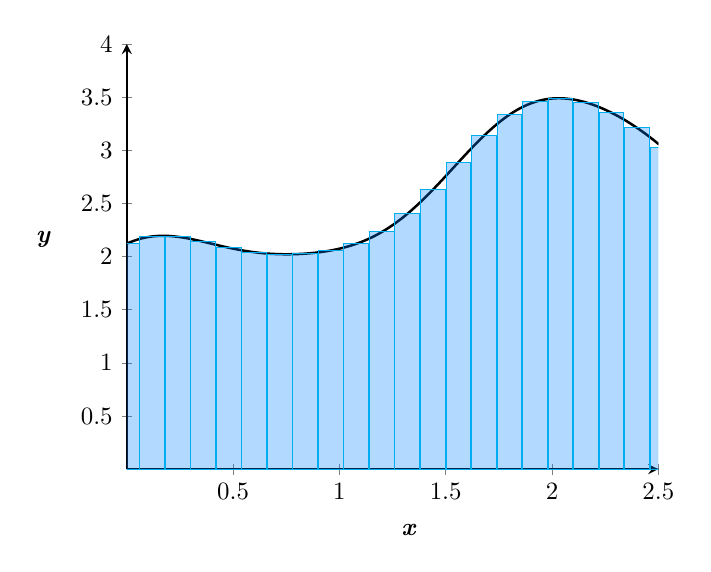
\begin{tikzpicture}[scale=0.9,
    declare function={
    % f(\x)=(\x^2)+9*\x+7;
        f(\x)=2+cos(deg(\x-2))+cos(deg(3*\x))/2+sin(cos(5*\x))/8 + cos(deg(7*\x))/28;
    }
]
\begin{axis}[
    axis lines = middle,
    xtick ={0.5, 1.0, 1.5, 2.0, 2.5, 3.0, 3.5},
    ytick ={0, 0.5, 1, 1.5, 2.0, 2.5, 3, 3.5, 4, 4.5, 5, 5.5},
    % xticklabels = {$a=x_0$,$x_1$,$x_2$,$x_3$, $\ldots$, $x_{n-1}$,$x_n=b$},
    ymin = 0,
    ymax = 4,
    xmin = 0,
    xmax = 2.5,
    x=3cm,y=1.5cm,
    axis line style = thick,
    xlabel style={at={(.5,0)},above right,yshift=-30pt},
    ylabel style={at={(0,.5)},above right,xshift=-40pt},
    xlabel={$\textit{\textbf{x}}$},
    ylabel={$\textit{\textbf{y}}$},
    % extra x ticks={1.3,1.85,2.2,2.7,3.2,3.75}
]

\addplot [
    % domain=1:4,
    samples=300,
    % line width=1pt,
    % fill=red, draw=none,
    % fill opacity=0.1
] {f(x)} \closedcycle;

\addplot [
    domain=0:5,
    samples=300,
    line width = 1pt, black] {f(x)};

\addplot[ybar, bar width=10pt, domain=1:4,samples at={0, 0.12, 0.24, 0.36, 0.48, 0.60, 0.72, 0.84, 0.96, 1.08, 1.20, 1.32, 1.44, 1.56, 1.68, 1.80, 1.92, 2.04, 2.16, 2.28, 2.40, 2.52, 2.64, 2.76, 2.88, 3.00, 3.12, 3.24, 3.36, 3.48}, fill=blue!50!cyan,fill opacity=0.3, draw=cyan]
  {f(x)};
\end{axis}
\end{tikzpicture}
\end{center}
\caption{Midpoint-Riemann Approximation of a Function}
\label{fig:riemannf}
\end{figure}

Allow the user to enter a radius $r$ and a delta $\Delta$, then compute a left/right-Riemann approximation of the area of a circle. Hint: if you compute the left/right-Riemann approximation of one quadrant, you can very easily obtain an approximation of the total circle area. We illustrate this hint in Figure ~\ref{fig:circlearea} where $\Delta=0.5$ and its radius $r=2$. Note that the approximated area will vary based on the chosen Riemann approximation.\footnote{A left-Riemann sum under-approximates the area, whereas a right-Riemann sum provides an over-approximation. A midpoint approximation uses the average between the left and right approximations. It should be noted that, in the general case, these statements do not hold as they depend on the interval we integrate our function over.} Further note that no calculus knowledge is necessary to solve this exercise.

\begin{figure}[H]
\begin{center}
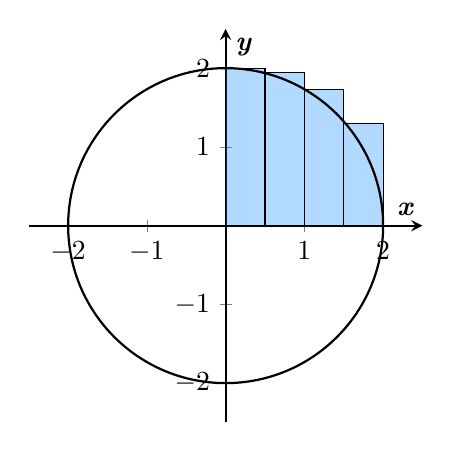
\begin{tikzpicture}
\begin{axis}[
    axis lines = middle,
    xtick ={-3,-2,-1,0,1,2,3},
    ytick ={-3,-2,-1,0,1,2,3},
    % xticklabels = {$a=x_0$,$x_1$,$x_2$,$x_3$, $\ldots$, $x_{n-1}$,$x_n=b$},
    ymin = -2.5,
    ymax = 2.5,
    xmin = -2.5,
    xmax = 2.5,
    x=1cm,y=1cm,
    axis line style = thick,
    xlabel={$\textit{\textbf{x}}$},
    ylabel={$\textit{\textbf{y}}$},
    % extra x ticks={1.3,1.85,2.2,2.7,3.2,3.75}
]
\end{axis}

  \draw[fill=blue!50!cyan,fill opacity=0.3] (2.5,2.5) rectangle (3,4.5);
  \draw[fill=blue!50!cyan,fill opacity=0.3] (3.0,2.5) rectangle (3.5,4.44);
  \draw[fill=blue!50!cyan,fill opacity=0.3] (3.5,2.5) rectangle (4.0,4.23);
  \draw[fill=blue!50!cyan,fill opacity=0.3] (4,2.5) rectangle (4.5,3.80);
\draw[thick] (2.5,2.5) circle (2);
\end{tikzpicture}

\end{center}
\caption{Right-Riemann Approximation of a Function}
\label{fig:circlearea}
\end{figure}

\subsubsection*{Bitwise Operations and Flags}

At their core, computers understand nothing more than zeroes and ones, i.e., \textit{binary values}\index{binary}. Decimal numbers are nothing more than an abstraction for humans.

For instance, consider the number $5_{10}$, where $n_{10}$ informs us that $n$ is a base ten number, or decimal. How can we represent the same idea, but in binary? Recall from Chapter~\ref{chapter-maths} that there are ten digits: $0$ to $9$. In binary, there are only two possible values: $0$ and $1$. So, intuitively, how can we encode zero? The simplest answer is to say that $0_{10} = 0_2$, where $n_{2}$ lets us know that $n$ is a base two number, or binary. What about one? $1_{10}=1_{2}$. We run into a problem with $2_{10}$ because $2$ is not a valid value in binary! So, like we do in decimal when we reach ten, we simply roll the next value over by one and reset the right position to zero. Thus, $2_{10} = 10_{2}$. This pattern cycles ad infinitum, and so therefore $5_{10} = 101_{2}$. $35_{10} = 100011_{2}$. Perhaps we should write a function that converts a positive decimal value into a corresponding binary value string. E.g., $35_{10} =$ \texttt{"100011"}. Though, there is an issue: we do not know how many bits a decimal number uses, right? Wrong! Logarithms are to the rescue. If we take $\log_{2}{35}$, we get approximately $5.192$. We saw that it takes six bits, or binary digits, to represent $35_{10}$ in binary. It may be tempting to round our decimal value to the next closest integer with the ceiling function. This will not work, however, because it fails to account for exact powers of two. E.g., $\lceil{}\log_{2}{16}\rceil{}=4$, but $16_{10}=10000_{2}$, meaning we should add one, then take the floor of the result, i.e., $\lfloor{}\log_2{n}+1\rfloor{}$. We use the \texttt{math.h} header for the relevant functions.

\begin{cl}[main.c]{Positive Decimal Values to Binary Function Stub}\begin{lstlisting}[language=MyC]
char *decimal_to_binary(int n) {
 // Negatives are impossible with this function.
 if (0 > n) {
  EPF("decimal_to_binary: n must be > 0!\n");
  exit(EXIT_FAILURE);
 }
 // Handle zero case.    
 else if (0 == n) { // TODO. } 
 else             { // TODO. }
 return NULL;
}
\end{lstlisting}\end{cl}

This function should return a dynamically-allocated string representing the converted value in binary. The (any base) logarithm of zero is undefined, so we need to manually account for this case. Returning a string literal is not appropriate since string literals are not dynamically-allocated; a duplicated string literal is therefore warranted!

\begin{cl}[main.c]{Handling Zero Case in Decimal-to-Binary Conversion}\begin{lstlisting}[language=MyC]
char *decimal_to_binary(int n) {
 char *result = NULL;
    
 // Negatives are impossible with this function.
 if (0 > n) {
  EPF("decimal_to_binary: n must be > 0!\n");
  exit(EXIT_FAILURE);
 }
 // Handle zero case.    
 else if (0 == n) {
  result = strdup("0");
 } else { // TODO. }

 return result;
}   
\end{lstlisting}\end{cl}

Now comes the interesting case. Using the logic on logarithms and bits from earlier, we know how many elements should be in our string: the number of required bits plus one for the \texttt{NUL}-termination character.

\begin{cl}[main.c]{Handling Zero Case in Decimal-to-Binary Conversion}\begin{lstlisting}[language=MyC]
char *decimal_to_binary(int n) {
 char *result = NULL;
 (*;\textcolor{lightgray}{$\ldots$};*)
 if (0 > n) { (*;\textcolor{lightgray}{$\ldots$};*) }
 // Handle zero case.    
 else if (0 == n) { (*;\textcolor{lightgray}{$\ldots$};*) } 
 else {
  int no_bits = (int) floor(log2(n) + 1);
  result = malloc(no_bits + 1);
  (*;\textcolor{lightgray}{$\ldots$};*)
 }
 return result;
}   
\end{lstlisting}\end{cl}

We now need to traverse through the number and determine, at each binary digit, whether it is a one or zero, and concatenate the relevant character. How do we do this? We need to introduce bitwise operators, or operations that act on bits, as the name suggests.\footnote{We could use the modulo operation, but that is not as fun!}

First, we will discuss bitwise OR\index{bitwise OR}, denoted as `$|$'. When we take the bitwise OR of two integer values $m$ and $n$, we create a result whose bits are set if the corresponding bit is set in at least $m$ or $n$. For instance, take $145_{10}\;|\;91_{10}$. The binary representation of these values is $10100001_{2}\;|\;01011011_{2}$. All we need to do is see if a bit is set at each position in the binary value, leading to $11011011_{2}$ or $219_{10}$. 

Up next is bitwise AND\index{bitwise AND}, denoted as `$\&$'. Bitwise AND is similar to OR with the exception that the corresponding bit must be set in both $m$ and $n$. Using the numbers from before, $145_{10}\;\&\;91_{10}$ is $10001_{2}$ or $17_{10}$.

Now, there is bitwise XOR\index{bitwise XOR}, denoted as `\^{}'. Bitwise XOR has its corresponding bits set if exactly one of $m$ or $n$ has the bit set. Thus, $145_{10}$ \^{} $91_{10}$ is $11001010_2$ or $202_{10}$.

Finally, we have bitwise NOT\index{bitwise NOT}, otherwise known as one's complement denoted by `$\bt{}$'. Bitwise NOT flips all bits in a number, meaning it is a one-place operator. Though, bitwise NOT has a very special property that must be explained: it does not account for only the bits used in its representation, but rather also leading zeroes.\footnote{While all bitwise operators operate on the entire operand, we were operating under the assumption that our values were stored as 8-bit integers in the preceding examples and explanations on the binary bitwise operators.} For instance, suppose we store $91$ in a 32-bit \texttt{int}. This, to the program/computer, looks like $00000000\;00000000\;00000000\;01011011_{2}$. When we perform a bitwise NOT on said value, we flip all bits, including any leading zeroes. Thus, we end up with $11111111\;11111111\;11111111\;10100100_{2}$, which is a number over four billion, right? Technically yes, but according to C, this is not correct. According to the program, we stored this value as a \textit{signed integer}, meaning it has a single bit denoting whether it is positive or negative. The sign bit is the most-significant bit, i.e., the ``farthest-left bit''. So, rather than representing numbers from 0 until $2^{32}\;-\;1$, we represent numbers from $-2^{31}$ until $2^{31}\;-\;1$. Though, this still does not necessarily answer the question—what is $\bt{}91$? ``It certainly is not negative two billion'', is a correct response. In order to accurately represent a negative number, C uses the two's complement representation. We stated that bitwise NOT uses one's complement, which simply flips every bit. Two's complement, on the other hand, flips every bit except the sign bit and adds one to the result. Thus, taking the previous result of $11111111\;11111111\;11111111\;10100100_{2}$ and flipping every bit except for the sign bit results in $10000000\;00000000\;00000000\;01011011_{2}$. Finally, we add one to the number to get $10000000\;00000000\;00000000\;01011100_{2}$, which is equivalent to $-92_{10}$. An astute reader may notice that this is just adding one to $91_{10}$ and negating the result. Once again, this is a correct observation! Thus, bitwise NOT adds one and negates its value.

Let us briefly return to the \texttt{decimal\_to\_binary} function. We know that we can use bitwise AND to determine whether the least significant bit is set via $n\;\&\;1$. Though, how can we test the next bit, i.e., the second-least significant bit, and so on? That brings us to the topic of bit-shifting operators.

Bitwise shifting\index{bitwise shift} is very intuitive from both a computer's and human's perspective. When we bit shift a number, it means that we take its binary digits and, literally, shift them either to the left or to the right. As an example, $111011101_{2}=477_{10}$ bit shifted to the left becomes $1110111010_{2}=944_{10}$. Conversely, bit shifting to the right becomes $11101110_{2}=238_{10}$. Thus, shifting left adds a trailing zero and shifting right adds a leading (but implicit) zero.\footnote{Bitwise right-shifting throws a wrench into the complexity by dealing with sign-extension. That is, suppose we bitwise right-shift a negative number. The sign bit is set, and as such, we carry that into the shifted result. E.g., $-64_{10}$, as a 32-bit integer, is $11111111\;11111111\;11111111\;11000000_{2}$, but shifting it to the right by $2_{10}$ gets us $11111111\;11111111\;11111111\;11110000_{2}$, or $-16_{10}$. Moreover, if we shift a positive integer to the left, we might accidentally overwrite the sign bit with a one! E.g., $16_{10}$, as a 32-bit integer, is $00000000\;00000000\;00000000\;00010000_{2}$, but shifting it to the left by twenty eight bits gets us $10000000\;00000000\;00000000\;00000000_{2}$}, which is $-1_{10}$ after performing two's complement arithmetic. Another perspective is to say that shifting a positive integer to the left by one multiplies said integer by two, and shifting to the right divides said integer by two (using integer division). It is better to say, though, that shifting either multiplies or divides the number by a power of two. E.g., shifting by three multiplies or divides the value by $2^{3}=8$.

Using this logic, we can finish our \texttt{decimal\_to\_binary} function. That is, we check each bit of our number using bit shifting and bitwise AND. If the corresponding bit is set, we add the character \texttt{`1'} to the character array and otherwise add \texttt{`0'}.

\begin{cl}[main.c]{Integrating Bitshifting}\begin{lstlisting}[language=MyC]
char *decimal_to_binary(int n) {
 char *result = NULL;
 (*;\textcolor{lightgray}{$\ldots$};*)
 else {
  int no_bits = (int) floor(log2(n) + 1);
  result = malloc(no_bits + 1);
  for (int i = 0; i < no_bits; i++) {
   if (0 == ((n >> i) & 1)) {
    result[i] = '1';
   } else {
    result[i] = '0';
   }
  }
  result[no_bits] = '\0';
 }
 return result;
}   
\end{lstlisting}\end{cl}

Interestingly, these bitwise operations are applicable to boolean values as well. E.g., $\texttt{true}\;\mathbin{|}\;\texttt{true}$ is nothing more than $1\;\mathbin{|}\;1$. Similarly, $\texttt{false}\;\mathbin{\&}\;\texttt{true}$ is nothing more than $0\;\mathbin{\&}\;1 = 0$. A purpose of using bitwise operations, however, is to combine multiple boolean values into one integer. Consider a file on a computer. Files have different permission properties, i.e., information that says who can access and mutate a file or its contents. Suppose our computer has three user classifications: file owners, groups, and others. The user who created a file, as its name suggests, is the file owner. We categorize a collection of individuals under some identifier, e.g., ``students'' or ``faculty'' as a group. Finally, there are others, which accounts for all users that are not the owner nor part of a group. Further imagine that a file has three permission types: read, write, and execute. If we had to keep track of individual booleans, we would have to worry about altering the state of nine booleans for every file! Even if we store these in an array, it is still cumbersome. Bitwise operations are our friend. If we use a ``short'' data type, we have sixteen bits to work with—more than enough. We designate the three least significant bits for ``other user'' permission, the next three are for ``group'' permission, and the following three bits are for ``owner'' permission. Correspondingly, we use define to give names to these bit positions.

\begin{cl}[]{}\begin{lstlisting}[language=MyC]
#define OTHER_EXEC  0x0001
#define OTHER_WRITE 0x0002
#define OTHER_READ  0x0004

#define GROUP_EXEC  0x0008
#define GROUP_WRITE 0x0010
#define GROUP_READ  0x0020

#define OWNER_EXEC  0x0040
#define OWNER_WRITE 0x0080
#define OWNER_READ  0x0100
\end{lstlisting}\end{cl}

Because each permission has exactly one set bit, as demonstrated by using powers of two, we can combine file permissions. For instance, if we want to say that a file can be read, written, and executed by only the owner, we use a bitwise OR to set the three respective constants.

\begin{cl}[]{}\begin{lstlisting}[language=MyOutput]
perm = OWNER_READ | OWNER_WRITE | OWNER_EXEC;
\end{lstlisting}\end{cl}

Which translates, in hexadecimal, to $\texttt{perm} = 0001_{16}\;|\;0002_{16}\;|\;0004_{16} = 01C0_{16}$.

If we want to check to see if a file has a certain permission, we use bitwise AND to check if the corresponding bit is set. Essentially, we want to see if the result of a bitwise AND with the relevant position is a non-zero value (because if we bitwise AND two numbers, only sharing set bits are set in the result). For example, checking ``perm'' to see if \texttt{GROUP\_EXEC} is set looks like (\texttt{perm \& GROUP\_EXEC}). In C, as we have mentioned, a conditional resolves non-zero values as true, meaning that as long as this is a non-zero value, it indicates that the flag is set. To set a flag, we use bitwise OR: \texttt{perm = perm | GROUP\_EXEC}, or the less verbose augmented assignment operator: \texttt{perm |= GROUP\_EXEC}. To disable a flag, we use bitwise AND combined with bitwise NOT: \texttt{perm = perm \& \bt{}GROUP\_EXEC}, or \texttt{perm \&= \bt{}GROUP\_EXEC}. The reason this works is because, if \texttt{GROUP\_EXEC} is $0008_{16}$, then \texttt{\bt{}GROUP\_EXEC} = $\text{FFF}7_{16}$. So, bitwise AND-ing any number with this bit toggled will disable it, and if it is already disabled, nothing happens. To ``toggle'' a bit, we use bitwise XOR: \texttt{perm \^{}= GROUP\_EXEC}. Again, if the bit is set in \ttt{perm}, because \texttt{GROUP\_EXEC}'s bit is always trivially set, that bit in \ttt{perm} is disabled due to the properties of XOR. If it is disabled because of XOR properties, it becomes set (i.e., 0 \^{} 1 = 1).

Another reason to work with bitwise operations comes through how colors are (typically) represented in computers. Most often, computers store colors as \textit{alpha-red-green-blue} integers, since as we have repeatedly mentioned, computers only understand numbers at their core. Namely, a 32-bit integer stores the data associated with a color where the most-significant byte stores the alpha channel, the next byte stores the red channel, the next stores the green, and the least-significant byte stores the blue channel. A channel, as suggested, is a value between 0 and 255 inclusive. Often times, colors are represented using hexadecimal as a means of shortening the notation. E.g., \texttt{0xffff00ff} represents a color whose alpha channel is $255$, red is $255$, green is $0$, and blue is $255$. It may be tempting to say that this is a fully-opaque purple color since mixing red and blue colors gets us purple. In terms of ARGB, though, this is not correct! It is, in fact, magenta. Why do we care about this, though? We can extract individual channels of an ARGB value using bitshifting and bitwise AND. For instance, to extract the red channel from an ARGB value $c$ requires us to bit shift the value down by $24$ and perform a bitwise AND on $255$, i.e., $(c\;\gg\;24)\;\&\;255$.

\exercise{5}{chapter-interpretation1}{Jef Poskanzer invented the PPM image file format in the late 1980's~\cite{ppm}. Its advantages over other image file formats include its listing of pixel data as explicit RGB values. PPM files also specify the image dimensions. For example, the following lines describe a $2 \times 3$ (pixel) image with red, green, and blue pixels in the first row, followed by blue, green, and red pixels in the second.}
\begin{verbatim}
P3
2 3
255
255 0 0 0 255 0 0 0 255
0 0 255 0 255 0 255 0 0
\end{verbatim}
Write two functions: \ttt{compress} and \ttt{decompress}. The former receives a two-dimensional array of integers corresponding to the RGB pixels of a PPM file. Its job is to create a new two-dimensional array that condenses these byte values into 32-bit integers. For instance, the color values \ttt{255 0 0} are compressible into \ttt{ff0000$_{16}$} using bitwise operations. Use the following macro to retrieve the corresponding value of given RGB channels:
\begin{cl}[]{}
\begin{lstlisting}[language=MyC]
#define COLOR_RGB(R, G, B)    \
    ((((R) << 16) & 0xff0000) \
    | (((G) << 8) & 0x00ff00) \
    | ((B) & 0x0000ff))     
\end{lstlisting}
\end{cl}
The latter \ttt{decompress} function, on the other hand, does the opposite; it receives an array of integers and expands their values into separate red, green, and blue channels, returning a new two-dimensional array. Use the following macros to extract each color channel of an integer:
\begin{cl}[]{}
\begin{lstlisting}[language=MyC]
#define GET_RED(C) (((C) >> 16) & 0xff)
#define GET_GREEN(C) (((C) >> 8) & 0xff)
#define GET_BLUE(C) ((C) & 0xff)
\end{lstlisting}
\end{cl}
\noindent The following exercises will use an image of a praying mantis as shown in Figure~\ref{fig:pm.png}.\footnote{The image is authored by Rick van der Haar, provided by \ttt{unsplash}.}

\exercise{1}{chapter-interpretation1}{Design a \ttt{struct image} to hold (integer) pixel data, as well as its (the image) corresponding width and height. The pixel data should be the ``compressed'' integers as described previously. We provide a template as follows:}
\begin{cl}[]{}
\begin{lstlisting}[language=MyC]
typedef struct image {
 // TODO (you fill this in!).
} image;
\end{lstlisting}
\end{cl}

\exercise{3}{chapter-interpretation1}{Write a function \ttt{zero\_red}, which receives an image and returns a new image where the red channel of all pixels is set to zero (see Figure~\ref{fig:pmzerored}).}
\begin{figure}[H]
\centering
\begin{minipage}{.45\textwidth}
  \centering
  \includegraphics[width=.45\linewidth]{res/images/pm.png}
  \caption{Praying Mantis}
  \label{fig:pm.png}
\end{minipage}%
\centering
\begin{minipage}{.45\textwidth}
  \centering
  \includegraphics[width=.45\linewidth]{res/images/pmzerored.png}
  \caption{No Red Channel}
  \label{fig:pmzerored}
\end{minipage}%
\end{figure}

\exercise{3}{chapter-interpretation1}{Write a function \ttt{negative}, which receives an image and returns a new image where each color is converted to its negative counterpart. The negative of a color is the color created when each channel is subtracted from $255$ (see Figure~\ref{fig:pmnegative}).}

\exercise{3}{chapter-interpretation1}{Write a function \ttt{grayscale}, which receives an image and returns a new image where each color is converted to its grayscale counterpart. The grayscale of a color is the average of its color channels (see Figure~\ref{fig:pmgrayscale}).}
\begin{figure}[H]
\centering
\begin{minipage}{.45\textwidth}
  \centering
  \includegraphics[width=.45\linewidth]{res/images/pmnegative.png}
  \caption{Negative Image}
  \label{fig:pmnegative}
\end{minipage}%
\centering
\begin{minipage}{.45\textwidth}
  \centering
  \includegraphics[width=.45\linewidth]{res/images/pmgray.png}
  \caption{Grayscale Image}
  \label{fig:pmgrayscale}
\end{minipage}%
\end{figure}

\exercise{3}{chapter-interpretation1}{Write a function \ttt{swap\_red\_green}, which receives an image and returns a new image where each color has its red and green channels swapped (see Figure~\ref{fig:pmswaprg}). Then, write another function \ttt{swap\_green\_blue}, which swaps the green and blue channels of a given image (see Figure~\ref{fig:pmswapgb}).}
\begin{figure}[H]
\centering
\begin{minipage}{.45\textwidth}
  \centering
  \includegraphics[width=.45\linewidth]{res/images/pmswaprg.png}
  \caption{Red \& Green Swapped}
  \label{fig:pmswaprg}
\end{minipage}%
\centering
\begin{minipage}{.45\textwidth}
  \centering
  \includegraphics[width=.45\linewidth]{res/images/pmswapgb.png}
  \caption{Green \& Blue Swapped}
  \label{fig:pmswapgb}
\end{minipage}%
\end{figure}

\exercise{3}{chapter-interpretation1}{Write functions \ttt{mirror\_vert} and \ttt{mirror\_horz}, which return new images where the pixels are flipped along the $y$ and $x$ axes respectively (see Figures~\ref{fig:pmhorz} and~\ref{fig:pmvert}).}
\begin{figure}[H]
\centering
\begin{minipage}{.45\textwidth}
  \centering
  \includegraphics[width=.45\linewidth]{res/images/pmmirrorvert.png}
  \caption{Mirror Along $y$-axis}
  \label{fig:pmvert}
\end{minipage}
\centering
\begin{minipage}{.45\textwidth}
  \centering
  \includegraphics[width=.45\linewidth]{res/images/pmmirrorhorz.png}
  \caption{Mirror Along $x$-axis}
  \label{fig:pmhorz}
\end{minipage}%
\end{figure}

% \exercise{3}{chapter-interpretation1}{Write a function \ttt{mirror\_diag} that receives a CPD array and returns a new CPD array where its pixels are mirrored along the diagonal produced from the top-right to the bottom-left (see Figure~\ref{fig:pmdiagonal}). Assume the input CPD has dimensions $n \times n$.}
% \begin{figure}[H]
% \centering
% \begin{minipage}{.45\textwidth}
%   \centering
%   \includegraphics[width=.45\linewidth]{res/images/pmmirrordiag.png}
%   \caption{Mirror Along Diagonal}
%   \label{fig:pmdiagonal}
% \end{minipage}%
% \end{figure}

\exercise{3}{chapter-interpretation1}{Brightness and contrast are two properties of images, where brightness describes how close each pixel is to their maximum values, and contrast describes the distance between pixels in the image. In essence, the more contrast, the brighter the bright colors, and the darker the dark colors. These two properties are described by  $f(x) = \alpha{x}+\beta$, where $\alpha$ and $\beta$ represent contrast and brightness respectively. Contrast $\alpha$ is a multiplicative value, wherein an $\alpha \in (0,\; 1)$ lowers the contrast, and an $\alpha > 1$ increases the contrast. Brightness, on the other hand, is a linear additive value, wherein positive values of $\beta$ increase the brightness, and negative values decrease the brightness. The variable $x$ is a color channel. For this exercise, write a function \ttt{alter\_brightness\_contrast} that receives an $\alpha$ and $\beta$, modifying the corresponding components. You will need to write a function that ``clamps'' a value between $0$ and $255$ (see Figures~\ref{fig:pmbrighterm50} and~\ref{fig:pmbrighterc2x}).}
\begin{figure}[H]
\centering
\begin{minipage}{.45\textwidth}
  \centering
  \includegraphics[width=.45\linewidth]{res/images/pmbrighterm50.png}
  \caption{Brightness $-50$ Decrease}
  \label{fig:pmbrighterm50}
\end{minipage}%
\begin{minipage}{.45\textwidth}
  \centering
  \includegraphics[width=.45\linewidth]{res/images/pmbrighterc2x.png}
  \caption{Contrast $2$X Increase}
  \label{fig:pmbrighterc2x}
\end{minipage}
\end{figure}

\exercise{4}{chapter-interpretation1}{Write a function \ttt{clockwise} that receives an image and returns a new image where its pixels are rotated clockwise (see Figure~\ref{fig:pmclockwise}).}

\exercise{4}{chapter-interpretation1}{Write a function \ttt{clockwise\_four} that receives an image and returns a new image containing the pixel data of the original image rotated four times. The top-left quadrant should contain the original (image), the top-right is one clockwise iteration, the bottom-right is two clockwise iterations, and the bottom-left is three clockwise iterations (see Figure~\ref{fig:pmclockwisefour}).}

\begin{figure}[H]
\centering
\begin{minipage}{.45\textwidth}
  \centering
  \includegraphics[width=.45\linewidth]{res/images/pmclockwise.png}
  \caption{Clockwise Rotation}
  \label{fig:pmclockwise}
\end{minipage}%
\begin{minipage}{.45\textwidth}
  \centering
  \includegraphics[width=.45\linewidth]{res/images/pmclockwisefour.png}
  \caption{Four Cloclwise Rotations}
  \label{fig:pmclockwisefour}
\end{minipage}
\end{figure}

\exercise{5}{chapter-interpretation1}{Beno\^it Mandelbrot\index{Beno\^it Mandelbrot} discovered the \textit{Mandelbrot set}\index{Mandelbrot set} in the very early 1980's~\cite{mandelbrot}.\footnote{There is a common debate between which researcher(s) discovered the set; even though it is named after Mandelbrot himself, Brooks and Matelski published a paper with the equation and a text-representation of the fractal prior to Mandelbrot's publications~\cite{mandelbrotbrooks}.} To even begin discussing what the Mandelbrot set is, we need to very quickly introduce complex numbers. 

\textit{Complex numbers}\index{complex numbers} have a real and imaginary component, in which the imaginary component is multiplied by the imaginary constant $i$, or $\sqrt{-1}$. For example, $4\;+\;3i$ has a real component $4$ and an imaginary component $i$. We can add/subtract and multiply complex numbers as follows:}
\begin{align*}
    (a\;+\;bi) \pm (c\;+\;di) &= (a \pm c)\;+\;i(b \pm d)\\
    (a\;+\;bi) \cdot (c\;+\;di) &= (ac\;-\;bd)\;+\;i(ad\;+\;bc)
\end{align*}

\noindent Because this exercise is so involved, we will expand it into several sub-exercises.

\exercise{3}{chapter-interpretation1}{First, design a struct for working with complex numbers. This should, of course, contain two fields: a \ttt{double} for the real and a \ttt{double} for the imaginary.\footnote{The $i$ that accompanies the imaginary component is only present if we print the complex number; you should not store this value in any way inside the structure definition.} Then write the addition and multiplication functions over complex numbers. Finally, design the \ttt{abs} function, which returns the distance to the complex number in the plane from the origin. The absolute value of a complex number $c$ is the square root of the sum of its squared real and imaginary components, i.e., $\textit{abs}(c) = \sqrt{\textit{real}(c)^{2}\;+\;\textit{imag}(c)^{2}}$.}
\begin{cl}[]{Skeleton Code for Complex Numbers Implementation}
\begin{lstlisting}[language=MyC]
typedef struct complex {
 // TODO.
} complex;

/**
 * Initializes the given complex number with the given 
 * real and imaginary components.
 */
void complex_create(complex *c, double re, double im) { (*;\textcolor{lightgray}{$\ldots$};*) }

/**
 * Adds the complex number b to the complex number a.
 * We modify the components of a.
 */
void complex_add(complex *a, const complex *b) { (*;\textcolor{lightgray}{$\ldots$};*) }

/**
 * Multiplies the complex number b with the complex number a. 
 * We modify the components of a.
 */
void complex_mult(complex *a, const complex *b) { (*;\textcolor{lightgray}{$\ldots$};*) }

/**
 * Returns the absolute value of the given complex number.
 * This distance is from the complex components to (0, 0i).
 */
double complex_abs(const complex *a) { (*;\textcolor{lightgray}{$\ldots$};*) }
\end{lstlisting}
\end{cl}

\exercise{2}{chapter-interpretation1}{Design an exponentiation function over complex numbers. This may be defined using natural recursion. The exponent argument must be a positive integer.}

\exercise{2}{chapter-interpretation1}{Later on, we will need to normalize values from one interval to another. Namely, the Mandelbrot set exists between the values $[-2,\;2]$ on both axes of the complex plane. Design the \ttt{normalize} function, which receives five \ttt{double} values: a number to normalize, an old range, and a new range. The idea is, given a value $x \in [m,\;n]$ where $n\geq{m}$, we want to determine what value $x$ would be if it were between another range $[m',\;n']$. We present a sequence of examples as follows:}
\begin{clonarrow}[]{Normalization Function Examples}
\begin{lstlisting}[language=MyC]
/**
 * Normalizes a given value from one range to another.
 */
double normalize(double n, double old_min, 
                 double old_max, double new_min, 
                 double new_max) { (*;\textcolor{lightgray}{$\ldots$};*) }
                 
int main(void) {
 printf("%f\n", normalize(5, 1, 10, -1, 1));
 printf("%f\n", normalize(2.5, 1, 10, 0, 1));
 printf("%f\n", normalize(2.5, -5, 5, 1, 100));
 return 0;
}
\end{lstlisting}
\tcblower
\begin{lstlisting}[language=MyOutput]
0
0.25
75
\end{lstlisting}
\end{clonarrow}

With these details now covered, we can begin our discussion. The Mandelbrot set is a set of complex numbers such that, if we iterate over every point in the complex plane using some function $f(c)$, if $c$ diverges (to infinity), it is not part of the set. Conversely, if $f(c)$, after repeated iteration, appears to converge to a value, then it is in the set. We can then plot these points onto an image. The function $f$ that we are discussing is actually the following recursive definition, where $c$ is the complex number that we are iterating: $z_{n\;+\;1} = z_n\;+\;c$.

\exercise{2}{chapter-interpretation1}{Design the \ttt{mandelbrot\_iterate} function, which receives two complex numbers: $z$ and $c$, as well as an integer $m$ denoting the maximum number of possible iterations. Continuously apply the preceding recursive definition onto $z$ until we either exceed $m$ or the absolute value of $z$ is less than two. The former case means the value diverges, whereas the latter means the value converges and is, therefore, in the set. Return the number of iterations used to plot $c$. Note that, the higher value of $m$ we use, the more precise the Mandelbrot set.}

\exercise{4}{chapter-interpretation1}{
Design the \ttt{mandelbrot} function, which receives four \ttt{double} values representing the minimum and maximum values along the complex plane. For instance, to draw the entire fractal, we should pass $-2$, $-2$, $2$, $2$.\footnote{When we say ``the entire fractal'', we mean as opposed to a zoomed-in section of the fractal.} Our \ttt{mandelbrot} function normalizes the received $x$ and $y$ coordinates to the provided argument ranges, then invokes the iteration function. If the returned number of iterations exceeds the allowed maximum, set the pixel color to white. Otherwise, set it to black. Return these pixel values in an \ttt{image} struct. The desired image dimensions are up to you.}

\begin{cl}[]{Mandelbrot Skeleton Code}
\begin{lstlisting}[language=MyC]
#define IMAGE_WIDTH    ___
#define IMAGE_HEIGHT   ___
#define MAX_ITERATIONS ___

/**
 * Iterates the Mandelbrot set function using the given complex 
 * values of z and c. We iterate at most m times.
 */
int mandelbrot_iterate(complex *z, complex *c, int m) { 
 for (int i = 0; i < m; i++) {
  if (___) { return ___; } 
  else { z = ___; }
 }
 return ___;
}

/**
 * Constructs a PPM image of the Mandelbrot set. The parameters 
 * specify the starting and ending coordinates of the fractal "canvas".
 */
image *mandelbrot(double mincx, double mincy, 
                  double maxcx, double maxcy) { 
 image *img = ___;
 // Initialize the img fields accordingly.

 for (int x = 0; x < img->w; x++) {
  for (int y = 0; y < img->h; y++) {
   double cx = normalize(x, 0, IMAGE_WIDTH, ___, ___);
   double cy = normalize(y, 0, IMAGE_HEIGHT, ___, ___);

   complex z, c;
   complex_create(&z, cx, cy);
   complex_create(&c, cx ,cy);
   int num_it = mandelbrot_iterate(___, ___, MAX_ITERATIONS);
   img->pixels[y][x] = ___;
  }
 }
 return img;
}
\end{lstlisting}
\end{cl}

Interestingly, we can map colors to the Mandelbrot fractal using a variety of techniques. We present one possible to show what is possible with enough creativity in Figure~\ref{fig:fractal}.

\begin{figure}[H]
\centering
\includegraphics[width=.3\textwidth]{res/images/fractal.png}
\caption{Colored Mandelbrot Fractal}
\label{fig:fractal}
\end{figure}

\exercise{5}{chapter-interpretation1}{Digital data is transmitted via network communication. While it might seem straightforward to send an image to a friend, the process actually involves significant complexity on the networking end. In the upcoming exercises, we will replicate a basic networking system where hosts have the ability to exchange data with other hosts (this simulation grossly oversimplifies the complexities of network programming, but serves as a nice programming exercise).

We will be working with bits and bytes in this exercise, even more so than before. The standard C datatypes are subject to change based on the architecture and C compiler, which means that an \ttt{int} may not always store 32 bits. On the other hand, the \ttt{uint32\_t} type is guaranteed by the \ttt{stdint.h} library to always store the necessary bits for an unsigned 32-bit integer.}

A \textit{host}, in our network, has an identifier $\ttt{id}$ specified by a 32-bit integer. Hosts send and receive data \textit{packets}, which contain a header and a data field. Hosts store a stack of \ttt{packet} pointers, which reference packets where they (the specified host) are the intended recipient. The \textit{header} of a packet stores a preamble, a start-of-data byte, a destination host identifier, a source host identifier, and a length-of-packet. The preamble is a sequence of three bytes containing \ttt{00110011} \ttt{11001100} \ttt{00110011}, followed by the start-of-data \ttt{11001101}. The destination and source host identifiers are four-byte integers, and the length-of-packet is a two-byte value corresponding to the total number of bytes used for the given packet. The idea is that any arbitrary host will continuously read sequences of data and, if it intercepts a packet, it stores the packet in its stack only if it is the intended host. All packets are broadcasted to every device on the network, but are ``dropped'' if they are not the intended destination host.

\exercise{2}{chapter-interpretation1}{Design a \ttt{host} structure and type definition as specified above. Create the \ttt{host\_init} function, which receives a pointer to a host structure to initialize with a given identifier. In the interest of time, also write the \ttt{host\_add\_packet} function that adds a packet to the host's stack of packets.}

\begin{cl}[host.h]{Host Header Skeleton}
\begin{lstlisting}[language=MyC]
#ifndef HOST_H
#define HOST_H

#include <stdint.h>

typedef struct host host;

void host_init(uint32_t id);
void host_add_packet(host *h, packet *pkt);

#endif // HOST_H
\end{lstlisting}
\end{cl}

\begin{cl}[host.c]{Host Source Skeleton}
\begin{lstlisting}[language=MyC]
#include "host.h"

typedef struct host {
 ___;
 ___;
} host;

/**
 * Initializes a host with the given identifier.
 */
void host_init(host *h, uint32_t id) {
 // TODO.
}

/**
 * Adds a packet to the given host's message stack.
 */
void host_add_packet(host *h, packet *pkt) {
 // TODO.
}
\end{lstlisting}
\end{cl}

\exercise{2}{chapter-interpretation1}{Design the \ttt{packet} structure and type definition. It should include a nested structure definition for a \ttt{header}. From there, write the \ttt{packet\_init} function, which receives a pointer to a \ttt{packet}, a sender, a receiver, as well as an array of \ttt{uint8\_t} data, and initializes its fields as specified. Do not return the packet; only initialize the required fields. Remember to initialize the preamble and start-of-packet fields. }

\begin{cl}[packet.h]{Packet Header Skeleton}
\begin{lstlisting}[language=MyC]
#ifndef PACKET_H
#define PACKET_H

#include <stdint.h>

typedef struct packet packet;

void packet_init(packet *pkt, uint32_t send, uint32_t recv, 
                 uint8_t *data, uint16_t size_of_data);

#endif // PACKET_H
\end{lstlisting}
\end{cl}

\begin{cl}[packet.c]{}
\begin{lstlisting}[language=MyC]
#include "packet.h"

typedef struct packet {
 struct header {
  ___ preamble; ___ start_of_data; ___ send; 
  ___ recv; ___ size_of_data; 
 } hdr;
 ___ data;
};

/**
 * Initializes a packet with the given data and the other required fields.
 */
void packet_init(packet *pkt, uint32_t send, uint32_t recv, 
                 uint8_t *data, uint16_t size_of_data) { // TODO. }
\end{lstlisting}
\end{cl}

\exercise{3}{chapter-interpretation1}{Using the skeleton code in Listing 5.131, write the \ttt{forward} function, which receives a packet and forwards it, appropriately, to the intended recipient. The \ttt{forward} function should also receive an array of hosts and the number of hosts on the network.}

\begin{cl}[network.c]{Skeleton Code for Networking Exercise}
\begin{lstlisting}[language=MyC]
#include "host.h"
#include "packet.h"

#define NUM_HOSTS 5

void forward(packet *pkt, host *hosts, size_t num_hosts) {
 for (int i = 0; i < num_hosts; i++) {
  host curr_host = ___;
  if (___) {
   host_add_packet(___, ___);
  }
 }
}

int main(void) {
 // Declare 5 hosts.
 struct host hosts[NUM_HOSTS];
 host_init(&hosts[0], 3232238081);
 host_init(&hosts[1], 3232238126);
 host_init(&hosts[2], 3232238131);
 host_init(&hosts[3], 3232238224);
 host_init(&hosts[4], 3232238292);

 // A random packet with data.
 packet pkt;
 uint8_t data[15] = {72, 101, 108, 108, 111, 44, 32, 104, 
                     111, 115, 116, 32, 52, 54, 33};
 packet_init(&pkt, 3232238224, 3232238081, data, sizeof(data) + HEADER_SIZE);

 // Forward the packet.
 forward(&pkt, hosts, NUM_HOSTS);

 return 0;
}
\end{lstlisting}
\end{cl}

\exercise{4}{chapter-interpretation1}{Write an interface, either through standard input or terminal arguments, for the end-user to connect to a host and view its stored messages in the following format:}

\begin{verbatim}
Message 1/1
Sender: 192.168.10.144
Receiver: 192.168.10.1

Hello, host 46!
\end{verbatim}

To do this, write three functions: \ttt{get\_host\_id}, \ttt{get\_msg}, and \ttt{print\_message}. The two former functions receive pointers to strings and store the host identifier and message in those strings. The latter receives three strings representing the sender and receiver addresses, the message itself as a string, the message number, and how many messages the host who calls \ttt{print\_message} has stored inside its packets stack. The host identifier is printed as an \textit{IPv4} address, which is nothing more than a 32-bit integer separated into four octets.

\begin{cl}[network.c]{Skeleton Code for Utility Functions in Networking Exercise}
\begin{lstlisting}[language=MyC]
void print_msg(char *send, char *recv, char *msg, 
               size_t n, size_t msg_count) { // TODO. }

/**
 * Populates the pointer buffer with a string representing
 * the "IPv4 address" of the given value.
 * E.g., if id=3232238224, then *ptr="192.168.10.144"
 */
void get_ip(char **ptr, uint32_t id) {
 int ret = -1;
 if (NULL == *ptr) { ret = asprintf(ptr, ___, ___); } 
 else { ret = sprintf(*ptr, ___, ___); }
 if (0 > ret) {
  EPF("get_ip: failed to output host id to string\n");
  *ptr = NULL;
 }
}

/**
 * Populates the pointer buffer with the data contents. If
 * ptr is passed as NULL, allocate to it the number of 
 * characters necessary to store the data.
 */
void get_msg(char **ptr, uint8_t *data, size_t len) {
 if (NULL == *ptr) { *ptr = calloc(___, 1); }
 for (int i = 0; i < len; i++) {
  (*ptr)[i] = ___;
 }
}
\end{lstlisting}
\end{cl}

% \exercise{4}{chapter-interpretation1}{We can \textit{blur} an image by taking the average color of neighboring pixels. These neighboring pixels are called a \textit{kernel matrix}, and are used to apply effects such as blurring. Figure~\ref{fig:pmblur} demonstrates the effect of applying a $3\times{3}$ kernel blur to Figure~\ref{fig:pm.png}. As we see, it blurs the image but we lose a lot of detail. A \textit{Gaussian blur} takes a different approach; kernel pixels are closely related to the pixel $p$ they surround, so we should apply a stronger weight to kernel pixels that are closer to $p$ than those that are further away. The formula for computing the weight of a pixel $(x,\;y)$ is provided as follows using the $G$ function. Do not let this intimidate you, as the only variable missing is the standard deviation $\sigma$, or the ``spread'' of the data. A higher value of $\sigma$ means the blur is wider, and a lower $\sigma$ means the blur is narrower.}
% \[
% G(x,\;y) = \dfrac{1}{2\pi\sigma^2}e^{-(\frac{x^2+y^2}{2\sigma^{2}})}
% \]
% The value produced by $G$ is a weight to-be applied to the color values of a kernel pixel. For instance, if $G$ produces $0.75$ for a pixel $(x,\;y)$, then we apply a factor $0.75$ to the three color channels of the pixel at $(x,\;y)$. After computing the color of each kernel pixel, we find the average color of the kernel and apply it to its center pixel.

% Write an algorithm to produce the Gaussian blur of the praying mantis. It would be wise to write a function \ttt{gaussian}, which receives two pixel values $x$, $y$, and a standard deviation $\sigma$. It returns the result computed from the given Gaussian formula. You might also want to write a function \ttt{color\_average}, which receives an array of colors and returns an integer representing the average color.
